% mnras_template.tex 
%
% LaTeX template for creating an MNRAS paper
%
% v3.0 released 14 May 2015
% (version numbers match those of mnras.cls)
%
% Copyright (C) Royal Astronomical Society 2015
% Authors:
% Keith T. Smith (Royal Astronomical Society)

% Change log
%
% v3.0 May 2015
%    Renamed to match the new package name
%    Version number matches mnras.cls
%    A few minor tweaks to wording
% v1.0 September 2013
%    Beta testing only - never publicly released
%    First version: a simple (ish) template for creating an MNRAS paper

%%%%%%%%%%%%%%%%%%%%%%%%%%%%%%%%%%%%%%%%%%%%%%%%%%
% Basic setup. Most papers should leave these options alone.
\documentclass[fleqn,usenatbib]{mnras}

% MNRAS is set in Times font. If you don't have this installed (most LaTeX
% installations will be fine) or prefer the old Computer Modern fonts, comment
% out the following line
\usepackage{newtxtext,newtxmath}
\usepackage[flushleft]{threeparttable}
% Depending on your LaTeX fonts installation, you might get better results with one of these:
%\usepackage{mathptmx}
%\usepackage{txfonts}

% Use vector fonts, so it zooms properly in on-screen viewing software
% Don't change these lines unless you know what you are doing
\usepackage[T1]{fontenc}
\usepackage{setspace}

% Allow "Thomas van Noord" and "Simon de Laguarde" and alike to be sorted by "N" and "L" etc. in the bibliography.
% Write the name in the bibliography as "\VAN{Noord}{Van}{van} Noord, Thomas"
%\DeclareRobustCommand{\VAN}[3]{#2}
%\let\VANthebibliography\thebibliography
%\def\thebibliography{\DeclareRobustCommand{\VAN}[3]{##3}\VANthebibliography}


%%%%% AUTHORS - PLACE YOUR OWN PACKAGES HERE %%%%%

% Only include extra packages if you really need them. Common packages are:
\usepackage{graphicx}	% Including figure files
\usepackage{amsmath}	% Advanced maths commands
\let\Bbbk\relax
\usepackage{amssymb}	% Extra maths symbols
\usepackage[justification=centering]{caption}
\usepackage{float}
%% Reintroduced the \received and \accepted commands from AASTeX v5.2
%\received{June 1, 2019}
%\revised{January 10, 2019}
%\accepted{\today}
%% Command to document which AAS Journal the manuscript was submitted to.
%% Adds "Submitted to " the argument.

%\title[Short title, max. 45 characters]{Periodic X-ray Sources in the Galactic Bulge}
%\author{Bao \& Li}

\title[Periodic X-ray Sources in the Galactic Bulge]{Periodic X-ray Sources in the Galactic Bulge: Application of the Gregory-Loredo Algorithm}

\author[Bao \& Li]{
Tong Bao,$^{1,2}$\thanks{E-mail: baotong@smail.nju.edu.cn}
Zhiyuan Li,$^{1,2}$\thanks{E-mail: lizy@nju.edu.cn}
\\
% List of institutions
$^{1}$School of Astronomy and Space Science, Nanjing University, Nanjing 210046, China\\
$^{2}$Key Laboratory of Modern Astronomy and Astrophysics (Nanjing University), Ministry of Education, Nanjing 210046, China
}

% These dates will be filled out by the publisher
\date{Accepted XXX. Received YYY; in original form ZZZ}

% Enter the current year, for the copyright statements etc.
\pubyear{2015}

\begin{document}
\maketitle
%\correspondingauthor{August Muench}
%\email{greg.schwarz@aas.org, gus.muench@aas.org}
\begin{abstract}
We present the discovery of 23 X-ray periodic sources in the Limiting Window (LW), a low-extinction region in the Galactic bulge, locating 80' south of the Galactic center. Their luminosities range(${\rm 10^{31}-10^{33} ~erg ~ s^{-1}}$) and period distribution(mostly between 1 to 3 hour), indicate they are cataclysmic variables (CVs). Most of them are polars with relatively harder spectrum, suggesting an unusual sub-class of mCVs.
The brighter sources (6 out of 23 with L>$\rm 10^{32} ~erg~s^{-1}$) in this sample are more likely IPs, with mean $M_{WD}$ about 0.8 $M_\odot$.
We also proved that the Gregory-Loredo (GL) method used in this work has better sensitivity and data usage compared to the Lomb-Scargle (LS) method. In combination with the simulation and the geometry of accretion in CVs, we constrain the proportion of polars to X-ray sources in LW about 16\%, and the fraction of DNe is about 45\%, though with more uncertainty. Still, this discovery confirms the sub-type of unusual mCVs and provides a practical way to study the population about X-ray sources based on periodic modulation.
\end{abstract}

%% Keywords should appear after the \end{abstract} command. 
%% See the online documentation for the full list of available subject
%% keywords and the rules for their use.
%\keywords{Galaxy: bulge --- X-rays: stars --- X-rays: binaries}
\begin{keywords}
Galaxy: bulge --- X-rays: stars --- X-rays: binaries
\end{keywords}

\section{Introduction} \label{sec:intro}
Cataclysmic variables (CVs) are close binary including a white dwarf (WD) and a main-sequence or sub-giant companion, whose material could be accreted by Roche-lobe overflow or stellar wind. 
They can be divided into magnetic (mCVs) and nonmagnetic CVs (non-mCVs) according to their magnetic field strengths of WDs. In addition, the mCVs are split into polars ($P_{spin}/P_{orb}\simeq 1$) and IPs ($P_{spin}/P_{orb}\simeq 0.01-1$), depending on their level of synchronization. 
The evolution of CVs are driven by angular momentum losses (AML) to keep the period from expanding, which would made system detached. The existence of  "period gap" is caused by the change of mechanism for angular momentum losses.  The dominant AML mechanism in long-period
systems ($P_{orb}$ $\geq$ 3 hour) is "magnetic braking", whereas short-period CVs ($P_{orb}$ $\leq$ 2 hour) are  driven by gravitational radiation. Meanwhile, there is a minimum period of CVs, resulted from the mass-loss-induced loss of thermal equilibrium in companion star. The orbital period of CVs are mainly between 1 to 10 hours, making it suitable for X-ray timing analysis. 

It has been proved that the collective properties of CVs serve as great probe for dynamic interactions of their local environment, contributed from the high abundance of WDs in binaries. The effect would be remarkable only with extremely high stellar density (e.g. galactic center or global clusters \citep{2019ApJ...876...59C}) for us obtaining observable evidence in Hubble time. 
In addition to that, the individual properties of CVs provide hints for the accretion region and magnetic field, especially from their periodic variability.

It has been suggested that the thousands of X-ray sources in galactic center are magnetic cataclysmic variables, particularly intermediate
polars (IPs) \citep{2009ApJS..181..110M,2018ApJS..235...26Z}. Due to the lack of optical/infrared imaging and spectroscopy resulted from high extinction and source crowding, the direct identification of them has been really difficult.
In fact, even the presence and characteristics of the He II $\lambda 4686$ and H$\beta$ line have been often used to judge if a CV is magnetic or not, the proof is far from conclusive. In \cite{1992PhDT.......119S}, many IPs with weak H$\beta$ lines could not be identified from non-magnetic systems using this diagnostic. 
Hence the periodicity becomes a well recognized probe to study their population, because of their different features in periodic modulation (see Section~\ref{subsec:class}).  

In \citet{2003ApJ...599..465M}, eight periodic sources were identified as mCVs in galactic center region (GCR). Then for galactic bulge region, ten periodic sources were found by using Lomb-Scargle methods \citep{2012ApJ...746..165H}. They were believed as an unusual type of mCVs with harder spectra like IPs while their period distribution resembles that of polars. The research was based on the observation of low-extinction Window fields (LW), locating at $1^{\circ}4$ south of the Galactic center. Its rarity of avoiding the obscuration from molecular cloud deserved our deeper excavation of these X-ray sources. 
Besides, according to RK catalog \citep{2003A&A...404..301R}, the mCVs (mostly DNe) occupied 20\% in CVs sample, while for GCR, this fraction was reckoned over 30-40\% \citep{2016ApJ...826..160H,2012ApJ...746..165H}. The miss of non-mCVs demands reliable explanation from analyzing the properties of these sources. It may indicates that a large number of non-mCVs still awaits discovery since faint class can be always missed in flux-limited surveys.

In this work, we have taken full usage of \emph{Chandra} observations for LW. Meanwhile, the methods with more efficiency and the simulation with higher accuracy have been both operated. We explored the X-ray properties of 23 periodic sources (ten of them identified in \cite{2012ApJ...746..165H}). 
Section~\ref{sec:obs} describes the observation we used and the source detection process. Section~\ref{sec:methods} gives a brief overview about the main methods for period finding and focuses on the GL method we adopted in this work. 
Section~\ref{sec:results} is devoted to the confirmation of period finding results.
Section~\ref{sec:spectra} presents the spectra analysis for these periodic sources and the estimation of mass of WDs based on the Fe line diagnostic. 
The comparison with previous work , the identification for these periodic sources and the X-ray source population in the LW would be discussed in Section~\ref{sec:discussion}.

\section{X-ray Data Preparation} \label{sec:obs}
\subsection{{\it Chandra} observations} \label{subsec:xdata}
The LW towards the inner Galactic bulge has been extensively observed by {\it Chandra} with its Advanced CCD Imaging Spectrometer (ACIS).
A total of 13 ACIS-I observations were taken, three in 2005 and ten in 2008, resulting in a total exposure of 982 ks.
A log of these observations is given in Table \ref{tab:obsinfo}. 
A number of previous studies have made use of all or part of these observations, which primarily focused on the identification of discrete X-ray sources and the quantification of their statistical properties \citep{2009Natur.458.1142R,2009ApJ...700.1702V,2009ApJ...706..223H,2011MNRAS.414..495R,2012MNRAS.427.1633H,2013ApJ...766...14M,2016MNRAS.462L.106W}.


%\decimalcolnumbers
\begin{table*}
\centering
\caption{{\it Chandra} observations of the Limiting Window} \label{tab:obsinfo}
\centering
\begin{tabular}{ccccccc}
\hline
\hline
ObsID & Start Time & Nominal R.A. & Nominal Decl. &  Roll angle & Exposure & Mode\\
& UT & ($\circ$) & ($\circ$) & ($\circ$) & ks & \\ 
\hline
6362 & 2005-08-19 16:15 & 267.86875 & -29.58800 & 273 & 37.7 & FAINT \\
5934 & 2005-08-22 08:16 & 267.86875 & -29.58800 & 273 & 40.5 & FAINT \\
6365 & 2005-10-25 14:55 & 267.86875 & -29.58800 & 265 & 20.7 & FAINT \\
9505 & 2008-05-07 15:29 & 267.86375 & -29.58475 & 82  & 10.7 & VFAINT \\
9855 & 2008-05-08 05:00 & 267.86375 & -29.58475 & 82  & 55.9 & VFAINT \\
9502 & 2008-07-17 15:45 & 267.86375 & -29.58475 & 281 & 164.1 & VFAINT \\
9500 & 2008-07-20 08:11 & 267.86375 & -29.58475 & 280 & 162.6 & VFAINT \\
9501 & 2008-07-23 08:13 & 267.86375 & -29.58475 & 279 & 131.0 & VFAINT \\
9854 & 2008-07-27 05:53 & 267.86375 & -29.58475 & 278 & 22.8 & VFAINT \\
9503 & 2008-07-28 17:37 & 267.86375 & -29.58475 & 275 & 102.3 & VFAINT \\
9892 & 2008-07-31 08:07 & 267.86375 & -29.58475 & 275 & 65.8 & VFAINT \\
9893 & 2008-08-01 02:44 & 267.86375 & -29.58475 & 275 & 42.2 & VFAINT \\
9504 & 2008-08-02 21:23 & 267.86375 & -29.58475 & 275 & 125.4 & VFAINT \\
\hline
\end{tabular}
\end{table*}

We downloaded and uniformly reprocessed the archival data with CIAO v4.10 and CALDB v4.8.1, following the standard procedure\footnote{http://cxc.harvard.edu/ciao}.
The CIAO tool \emph{reproject\_aspect} was employed to align the relative astrometry among the individual observations, by matching the centroids of commonly detected point sources. ObsID 9502, which has the longest exposure (164.1 ks), served as the reference frame.
%The resultant accuracy in relative astrometry was typically better than $0\farcs1$.
The level 2 event file was created for each ObsID, with the arrival time of each event corrected to the Solar System barycenter (i.e., Temps Dynamique Barycentrique time) by using the CIAO tool \emph{axbary}.
We then constructed a merged event list, reprojecting all events to a common tangential point, [R.A., Decl.]=[267.86375, 29.58475].
The individual observations cover a similar field-of-view (FoV) due to their similar aimpoints and roll angles, as illustrated in Figure~\ref{fig:FoV} which displays the merged 2--8 keV counts image.
We have examined the light curve of each ObsID and found that the instrumental background was quiescent for the vast majority of time intervals.
Hence we preserved all the science exposures for source detection and subsequent timing analysis, taking the advantage of uninterrupted signals within each observation.  
\subsection{Source detection}\label{subsec:detect}
It is known that the LW suffers from moderate line-of-sight extinction, $N_{\rm H} \approx 7\times10^{21}{\rm~cm^{-2}}$ \citep{2011MNRAS.414..495R}, which obscures X-ray photons with energies $\lesssim$ 1 keV.
%there would be a large number of active binaries (AB) as foreground sources. ABs emit X-rays mainly below 2keV. Thus we use 2-8 keV to do source detection. 
Here we focus on sources prominent in the 2--8 keV band, which are most likely CVs located in the Galactic bulge. This will also facilitate a direct comparison with the CVs found in the Nuclear Star Cluster \citep{2018ApJS..235...26Z}, the line-of-sight column density of which, $N_{\rm H} \sim 10^{23}{\rm~cm^{-2}}$, is only transparent to photons with energies $\gtrsim$2 keV. 

Source detection was performed following the procedures detailed in \citet{2018ApJS..235...26Z}.
Briefly, we first generated for each observation an exposure map as well as point-spread function (PSF) maps with enclosed count fraction (ECF) of 50\% and 90\%. 
Both the exposure and PSF maps were weighted by a fiducial spectrum, which is an absorbed bremsstrahlung with a plasma temperature of 10 keV and a column density of $N_{\rm H}=10^{22}{\rm~cm^{-2}}$, representative of the X-ray sources in the LW. 
We then reprojected the individual exposure maps to form a stacked exposure map in the same way as for the counts images; the PSF maps were similarly stacked, weighted by the corresponding exposure map. 
Next, we employed {\it wavdetect} to identify discrete sources in the merged 2--8 keV counts image, supplying the algorithm with the stacked exposure map and the 50\%-ECF PSF map and adopting a false-positive probability threshold of $10^{-6}$. 
This resulted in a raw list of 847 independent sources in the 2--8 keV band. 
% {\bf [since photometry is involved in the timing anlysis, it's not a bad idea to describe the procedure here]}
%Since the goal of this paper is to identity periodic sources and we can only get robust periodic signal from relatively bright sources. The precise photometry correction for these sources are not necessary.

The source centroid derived from {\it wavdetect} was refined using a maximum likelihood method that iterates over the detected counts within the 90\% enclosed counts radius (ECR).
Starting from this step we consider the 1--8 keV band to maximize the signal from potential sources in the LW. 
Then, for each ObsID, source counts were extracted from the 90\% ECR, while background counts were extracted from a concentric annulus with inner-to-outer radii of 2--4 times the 90\% ECR, excluding any pixel falling within 2 times the 90\% ECR of neighboring sources.
Source crowding is not a general concern in the LW, but in a few cases the source extraction region was reduced to 50\% ECR due to otherwise overlapping sources. 
The total source and background counts were obtained by summing up the individual observations. 
Photometry (i.e., net photon flux and its error) for individual sources were calculated using the CIAO tool \emph{aprates}, which takes into account the local effective exposure, background and ECF. 
We consider a {\it significant detection} for a given source in a given ObsID if the photon flux is greater than 3 times the error. 
%For precisely processing, we exclude the contamination of nearby point sources and extended sources from background region by naked eyes. 
%Then this procedure was only applied for candidate periodic sources (as decribed in sec \ref{sec:results}) due to the manpower limit. 
We further define for each source an inter-observation {\it variability index}, $\rm VI=S_{max}/S_{min}$, where $\rm S_{max}$ and $\rm S_{min}$ are the maximum and minimum photon fluxes among all the significant detections, respectively. This implicitly requires significant detections in at least two observations.

\begin{figure*}
\centering
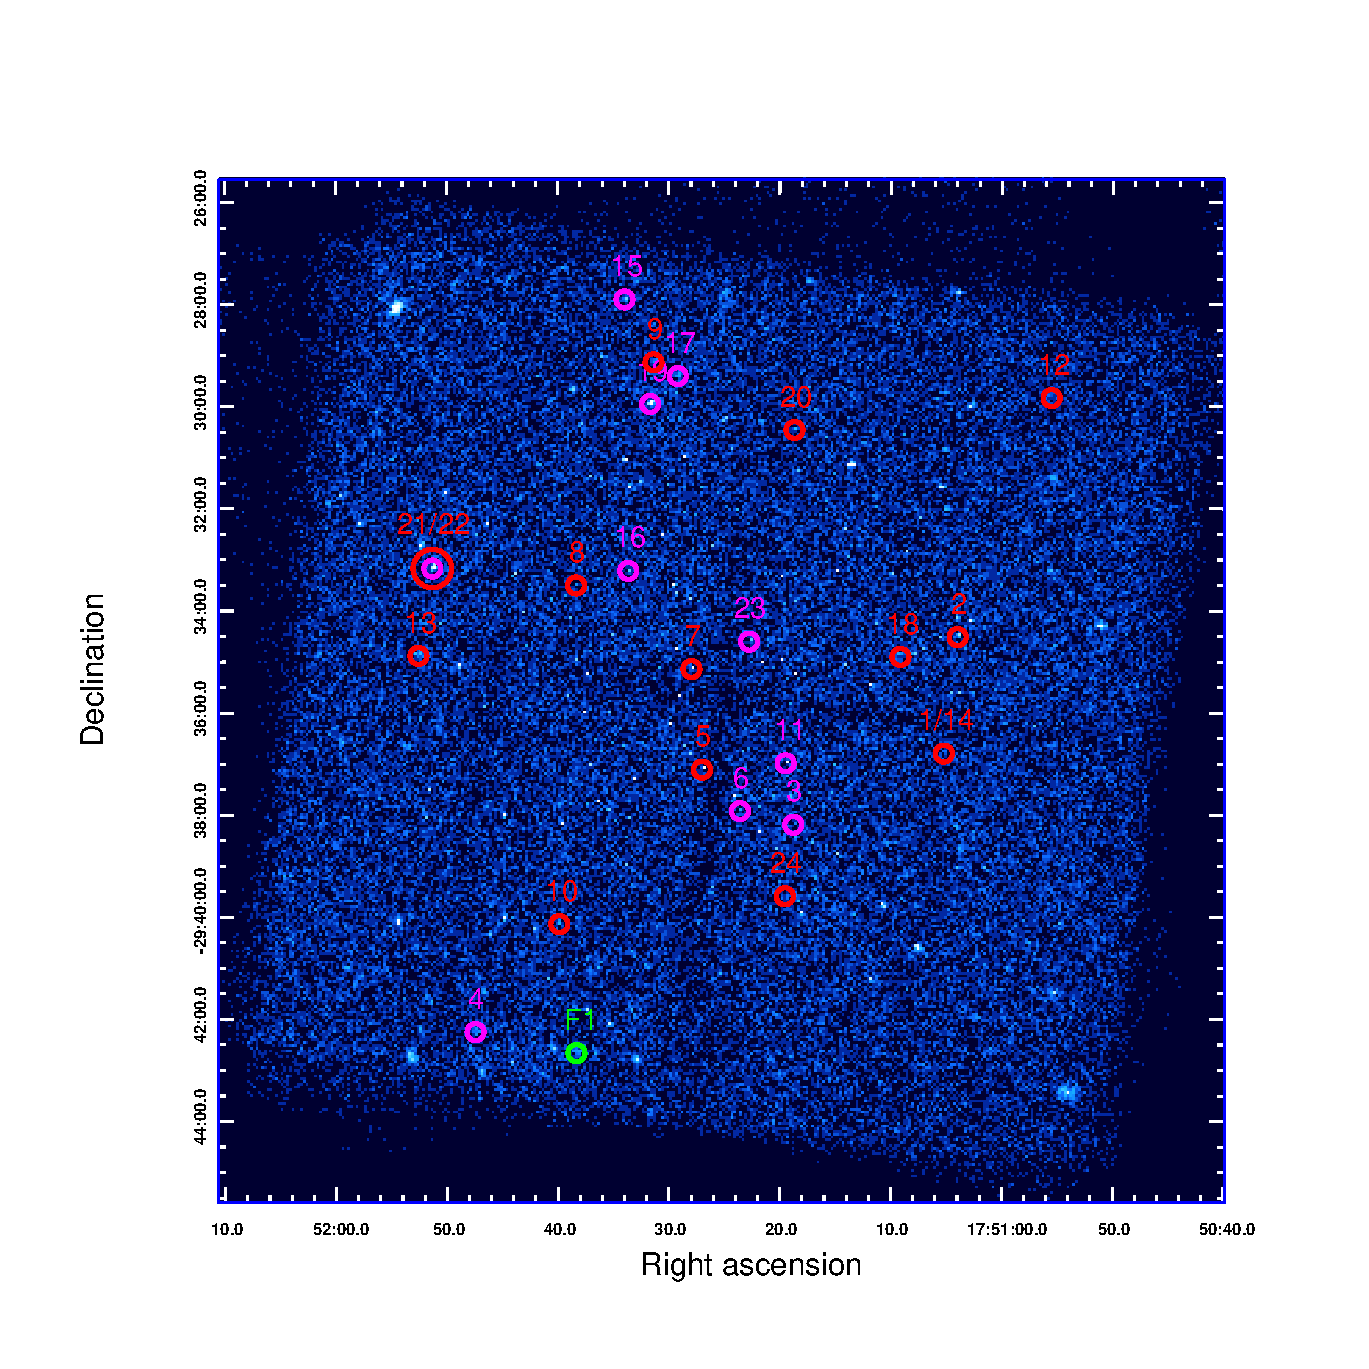
\includegraphics[scale=0.8]{./figure/LW/ds9.eps}
\caption{2--8 keV counts image of the Limiting Window, combining 13 {\it Chandra}/ACIS-I observations. Locations of the 23 periodic sources are marked with colored circles ({\it magenta}: ten sources previously reported by \citep{2012ApJ...746..165H}; {\it red}: twelve newly discovered in this work and belonging to the Galactic bulge; {\it green}: one newly discovered and located in the foreground). Source numbering is the same as in Table~\ref{tab:src}. In particular, 1/14 and 21/22 are the two sources each showing two periodic signals.}
\label{fig:FoV}
\end{figure*}

\section{Period Searching Method}\label{sec:methods}
In this section, we first provide our motivation of employing the Gregory-Loredo (GL) algorithm, followed by a brief description of its basic principles (Section~\ref{subsec:GL}). We then elucidate our application of the GL algorithm to the {\it Chandra} data of the LW (Section~\ref{subsec:appli}). This is complemented by a set of simulations to evaluate the detection (in)completeness of periodic signals (Section~\ref{subsec:simulation}).  

\subsection{The Gregory-Loredo Algorithm} \label{subsec:GL}
There exists in the literature a variety of period searching methods, which can be broadly divided into three categories according to their working principles. 

The most traditional method is based on Fourier transform and its power density spectra, which includes the classical Schuster periodogram \citep{1898TeMag...3...13S}, the Fourier analysis with unequally-spaced data \citep{1975Ap&SS..36..137D}, the correlation-based method \citep{1988ApJ...333..646E}, among others.

Another widely-used method seeks to fit the data with a periodic model in the frequency space, employing statistics such as least-squares residuals to define the likelihood function and then selecting the frequency that maximizes the likelihood. The famous Lomb-Scargle periodogram \citep[hereafter LS]{1976Ap&SS..39..447L,1982ApJ...263..835S} belongs to this category. Note that when adopting trigonometric functions, the least-squares method falls into the Fourier transformation category. Another variant is to replace the least-squares residuals with polynomial fits, such as that used in \citet{1996ApJ...460L.107S}.

The last category is the phase-folding method. For each trial period the time-tagged data is folded as a function of phase, and the best-fit period is found by optimizing the cost function through the frequency space. The cost function is designed to evaluate how much the phase-folded light curve deviates from constant.
Methods belonging to this category use diverse cost functions. Several widely known examples are the Epoch Folding (EF) algorithm \citep{1983ApJ...266..160L}, the Phase Dispersion Minimization \citep{1978ApJ...224..953S}, and the GL algorithm \citep{1992ApJ...398..146G}.

In X-ray observations, the detection of periodic signals is often involved with irregularly and sparsely sampled data. 
When working in frequency space, such a sampling can lead to spurious signals and hevay contamination to the real signal. Phase-folding methods, on the other hand, can avoid the effect of non-uniform data since the dead time does not enter the algorithm.
Moreover, the number of detected source counts is often only moderate. While one can in principle apply binning to create photometric light curve, it takes the price of potentially losing temporal information. Phase-folding methods, on the other hand, directly handle individual events, thus maximally incorporating the temporal information.

Most X-ray sources in the LW share the characteristics of irregular sampling and limited source counts. 
Therefore, it is appropriate to employ the GL algorithm, which applies the Bayesian probability theory to the phase-folded light curve, to search for periodic signals for the LW sources. We provide a brief overview of Bayes's theorem and the GL algorithm in Appendix \ref{GL}. 
The key of this algorithm is the multiplicity of the phase distribution of events,
\begin{equation}\label{multi}
W_m(\omega, \phi)={{N!}\over{n_1!\; n_2!\; n_3!\cdots {n_m}!}}.
\end{equation}
Here $N$ represents the total number of counts of a given source, 
%$m$ denotes the number of phase bins, and 
$n_i(\omega, \phi)$ is the number of events falling into the $i$th of $m$ phase bins given the frequency $\omega$ and the phase $\phi$, satisfying $\sum\limits_{i=1}^{m}n_i(\omega, \phi)=N$. 
The multiplicity is the number of ways that the binned distribution could have arisen by chance. It can be easily shown that the more the values of $n_i$ differ from each other, the smaller the multiplicity. In other words, the more the piecewise model defined the $m$ phase bins deviates from constant, the more likely there exists a periodic signal, the probability of which is inversely proportional to the multiplicity.  

In general, the GL algorithm takes the following steps:

(i) Compute the multiplicity for all sets of $(m,\omega, \phi)$ (Eqn.~\ref{multi}).

(ii) Given $m$, integrate over the $(\omega, \phi)$ space and calculate the so-called ``odds ratio'' using Bayes's theorem (Eqn.~\ref{A16}). The ``odds ratio'' determines the ratio of probabilities between a periodic model and a non-periodic (constant) model.

(iii) Sum up the normalized odds ratios of each $m$ to determine the probability of a periodic signal (Eqn.~\ref{A20}).
If this probability exceeds a predefined threshold (for instance, 90\%), a periodic signal is favored. 

(iv) Finally, compare all the odds ratios integrated over the $\phi$ space, finding the value of $\omega$ with the highest odds ratio, which then gives the period $P=2{\pi}/\omega$ (Eqn.~\ref{A21}).

%\section{Period searching procedure}\label{sec:timing}
\subsection{Application to the LW}\label{subsec:appli}
We apply the GL algorithm to search for periodic signals in the LW sources. 
For a given source, the 1--8 keV counts within the 90\% ECR of individual ACIS-I observations are extracted to form a time series.  
In addition, we supply for each source the information of ``epoch'', i.e., the start time and end time of each ObsID in which the source has at least one detected count. This information is used to compensate for the uneven distribution over the phase bins (see Eqn.~\ref{A17} for a detailed illustration). 
Since the GL algorithm determines the probability of a periodic signal against a constant light curve, there is no need to separately account for the background level, which is absorbed into the constant. 
Nevertheless, we have measured the local background (Section~\ref{subsec:detect}) for each periodic source as a consistency check (see Section~\ref{sec:results}). 
%Though we did source detection in 2-8 keV band to reduce the contamination from non-CV sources, here we still extracted photons from sources in 1-8 keV band to keep as more as possible source information. 
%Besides, in order to compensate for uneven distribution over the bins, we provide "epoch" for each source. The "epoch" offered the start time and end time of each observations covered the source with at least one counts in source region. See Eqn.~\ref{A17} in appendix for detailed illustration about the use of epoch. 
%For the sake of changing aimpoint, we used individual source extract region for different observations. Explicitly, the 90\% ECR aperture  whose radius defined by specific PSF map was applied for counts in that observation. Since the phase-folding method directly manipulated each photons and we could not distinguish background photon from source photon, the local background information were not provided for timing analysis. The combination of each source event list and the corresponding epoch were then employed as the input of GL method. 

As mentioned in Section~\ref{subsec:GL}, the GL algorithm folds the time series at a trial frequency (or period). 
In practice, the resolution of frequency must be compromised between accuracy and computational power. We choose the frequency range and frequency resolution for the following considerations.
%Here we generate the frequency resolution depended on the data timescale.

Ideally, the resolution of frequency should keep the phase-folded light curve nearly the same between two adjacent frequency, i.e., the phase bin of each photon should be unchanged.
For the data span in timescale T, the arrival time of photon $t_i$ (taking $t_1$=0), the changing angular frequency influence the phase of photon more as $i$ grows. The most "vulnerable" photon is the last photon arrived, whose arrival time is T, and the change of phase is
\begin{equation}\label{fi}
\begin{split}
	d\phi_{N}=&\phi_{N}^{'}-\phi_{N}\\
	=&[(\omega +d\omega) \cdot T-\lfloor (\omega +d\omega) \cdot T \rfloor] -[\omega \cdot T-\lfloor \omega \cdot T \rfloor]
\end{split}
\end{equation}
%\begin{equation}
%	\phi_{N}^{'}=(\omega +d\omega) \cdot T-\lfloor (\omega +d\omega) \cdot T \rfloor
%\end{equation}
%\begin{equation}
%	\phi_{N}=\omega \cdot T-\lfloor \omega \cdot T \rfloor
%\end{equation}
%\end{subequations}
\\
Assuming $\lfloor (\omega +d\omega) \cdot T \rfloor = \lfloor \omega \cdot T \rfloor$, ($\lfloor a \rfloor$means the integral part of a), then 
\begin{equation}
	d\phi_{N}=d\omega \cdot T
\end{equation}
In this work, we take 12 as the largest number of phase bins, that demands the change of photon phase should be smaller than the length of bin, i.e, ${1\over 12}\cdot 2\pi $, to guarantee the nearly non-change of phase-folded light curve. Although we can not ensure every photon to meet the requirement since its location in the same phase bin could be arbitrary. It would satisfy the situation at nearly perfect level if we keep the deviation of phase of last photon smaller than ${1\over 12}\cdot 2\pi $. As shown in Eqn.~\ref{dfi}
\begin{subequations}\label{dfi}
\begin{equation}
	d\phi_{N}=d\omega \cdot T< {1\over 12}\cdot 2\pi
\end{equation}
\begin{equation}
	d\omega < {{\pi}\over {6\;T}}
\end{equation}
\end{subequations}

The total span of 13 observation is about three years, i.e., $10^8$ s, so the resolution of angular frequency is $5\times 10^{-9}$. When the $\omega$ increases, corresponding the period decreases, the same resolution brings numerous discrete frequencies and raises running time greatly. Thus we used three different resolutions $10^{-7},10^{-8},10^{-9}$ in three period ranges $(300s,3000s),(3000s,10000s), (10000s,50000s)$. The ranges was chosen for the orbital period distribution of CVs, as shown in Figure \ref{fig:N_P}. There is a period gap in distribution at 2-3 hours, and a period minimum at about 70 minutes. Then the first range covers roughly the spin period of IPs, the other two ranges overlay the orbital period below and beyond the period gap respectively.

Generally, for each source, we provide the dataset for GL method. Then we got the most periodic signal with its probability in three period ranges. Taking 90\% as threshold to determine the periodicity, finally we choose all the candidate sources with at least one periodic signal.

\subsection{Detection completeness}\label{subsec:simulation}
For a given period searching algorithm, the detection rate depends on both the number of observed counts, the intrinsic shape of the light curve, as well as the observing cadence. 
To quantify the detection rate and hence gain insight on the nature of the periodic sources in the LW, we perform simulations following the merit of \citet{1998ApJ...498..666C}. 
Two functional forms of light curve are considered: a sinusoidal function and a piecewise function. While these are admittedly idealized shapes, they can represent realistic light curves, e.g., resulted from rotational modulation or eclipse. 

A sinusoidal light curve follows,
\begin{equation}
\lambda (t)=\lambda_0[1+A_{0}{\rm sin}(\omega t+\phi)], 
\label{eqn:sin}
\end{equation}
where $\omega = 2{\pi}/P$, $A_0$ is the relative amplitude of variation, and $\lambda_0$ is the mean count rate which may include contribution from a constant background. The phase $\phi$ can be arbitrarily set at zero.
For a direct comparison with observations, we relate $\lambda_0$ with the total number of counts, $C = \lambda_0 T$, where $T$ is the exposure time of a given observation. This holds since $T$ is typically much longer than the modulation period ($P$). 
The simulations are run with a selected number of parameters due to constraints in computational power. 
Specifically, we adopt $C$=50, 100, 200, 300, 400 and 500, $A_0$=0.5, 0.6, 0.7, 0.8 and 0.9, and $P$=554, 5540 and 45540 sec, resulting in a total of 6x5x3=90 combinations. 
The chosen periods are representative of the actually searched ranges (Section~\ref{subsec:appli}), whereas
the adopted total counts well sample the range of observed counts from the LW sources.

We thus simulate 100 light curves for each combination of parameters, taking into account Poisson errors and the exact start and end times of the 13 ACIS-I observations. The arrival time of each simulated count is further randomly modified by an amount of 3.2 sec to mimic the effect of ACIS frame time.
The simulated light curve is then searched for a periodic signal using the GL algorithm in the same manner as for the real data (Section~\ref{subsec:appli}).
We claim a valid detection if the found period has a detection probability greater than 90\% and its value consistent with the input period to within 1\%. 
%Besides, the harmonics have also been considered as valid detection  with the same threshold, i.e, the deviation between determined period and resonance cycle within 1\%.
We notice that for in a small fraction of simulate light curves of the shortest period (554 sec), the second harmonics (i.e., 2 times the true period) is detected with an even higher probability than the true period. We also consider such cases a valid detection as long as the true period fulfills the above criteria.
%In our simulation, the effect of harmonics only happens in the first period range due to the selection of parameter value, with fraction of harmonics detection about 20\%, concentrated at higher amplitude.
%For completeness, we ran the same process at $P$=4000 sec and $P$=20000 sec, adopting $C$=500 and $A_0$=0.9, and found there is no harmonics detection.

The detection rate for a given combination of parameters is taken to be the fraction of the 100 light curves having a valid detection. The top, middle and bottom panels of Figure \ref{fig:detection} show the result of the three test periods, respectively, in which several trends are apparent. 
First and intuitively, for a given period and amplitude, higher total counts would lead to higher detection rates, while for given total counts, a higher amplitude also leads to a higher detection rate. The simulation results confirm these expectations.  
Second, for the same total counts and amplitude, the detection rate is generally higher for a longer period.  
This can be understood as due to a statistical behavior in the 
multiplicity (see Eqn.~\ref{multi}), which has a lower value for a long period. This holds for both the sinusoidal and piecewise light curves. 
%it can be seen that the algorithm is nearly no bias of period, except a slight improvement of detection rate with increasing period. We exhaust every possibility to figure out the origin of improvement. After trial simulation, it turns out that statistically the multiplicity (Eqn.~\ref{multi}) has lower value with longer period, contributing to higher detection rate. Mathematically, this is due to the integral over time of counts rate (see Eqn.~\ref{eqn:sin}). The integral process brings about the value of deviation, between constant and variation, proportional to signal period because of the contribution of $w$ on denominator, resulting the negative association between multiplicity and period.
Lastly, for total counts of 50, the detection rate is almost always below 10\% regardless of the period and amplitude. 
%The periodic signal in this circumstance could be unreliable.
%With more counts, the detection rate can exceed 50\%, which is sufficient enough for period finding procedure. 
 
\begin{figure}
\begin{minipage}[b]{0.45\textwidth}
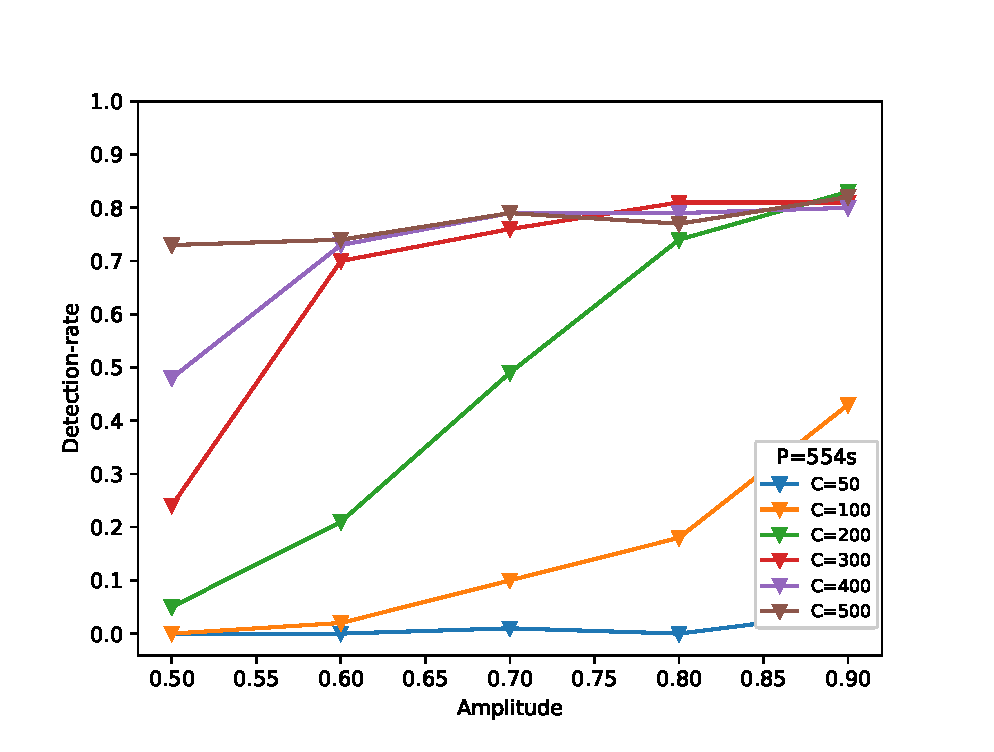
\includegraphics[width=\textwidth]{./figure/sim_LW/detection_554.eps}
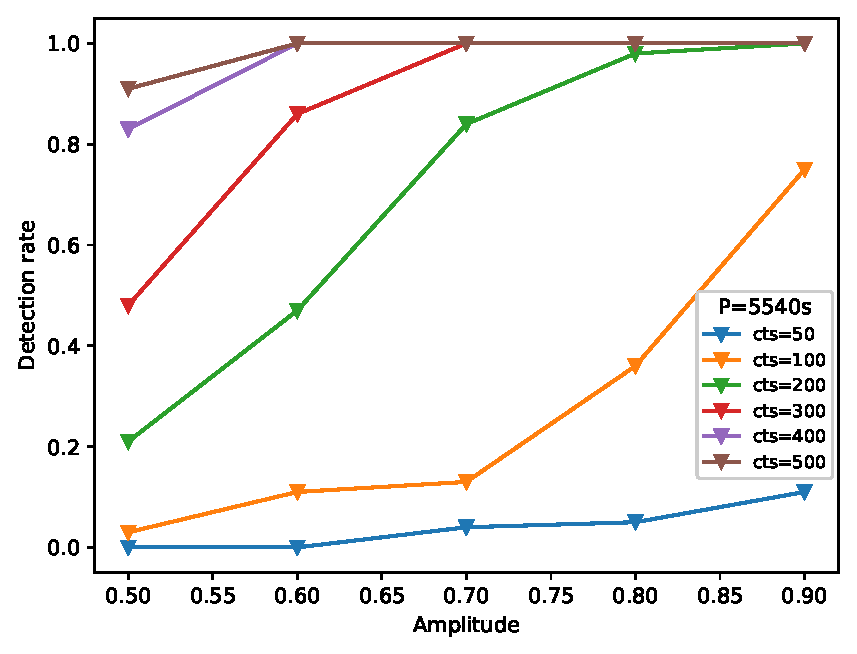
\includegraphics[width=\textwidth]{./figure/sim_LW/detection_5540.eps}
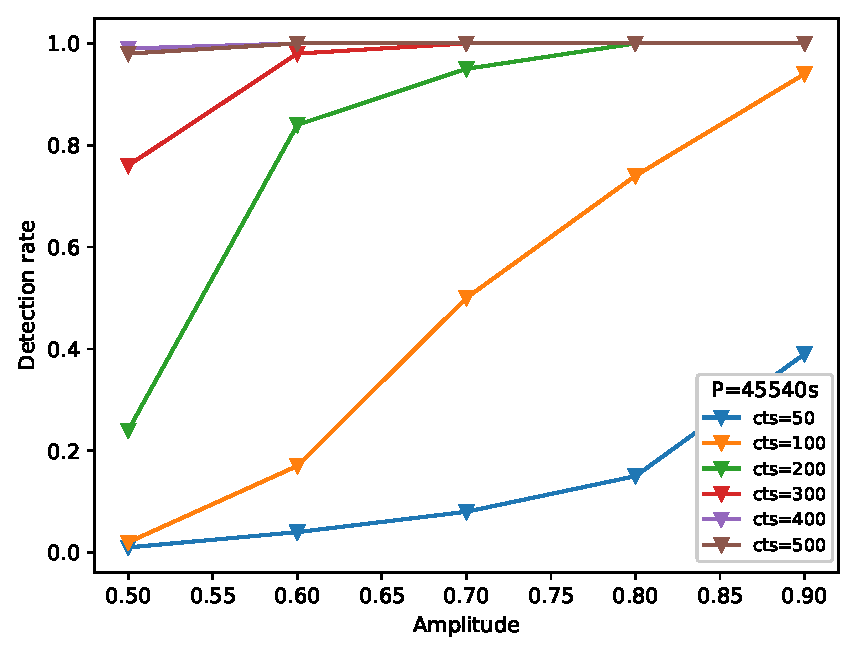
\includegraphics[width=\textwidth]{./figure/sim_LW/detection_45540.eps}
\end{minipage}
\caption{Detection rate obtained from simulation results for sinusoidal variation. The results of top, middle, bottom are respectively from modulation period as 554s, 5540s, 45540s. The other two parameters, $A_{0}$ and number of counts, are labeled by x-axis and colors. \label{fig:detection}}
\end{figure}

The piecewise function, which mimics an eclipse against an otherwise constant flux, takes the form of
\begin{equation}
\lambda(t)=
\begin{cases}
\lambda_0 & \text{$\phi(t) \in[0,(1-w)\pi)\cup ((1+w)\pi,2\pi]$},\\
f\lambda_0 & \text{$\phi(t) \in[(1-w)\pi,(1+w)\pi]$},
\end{cases}	
\end{equation}
where $w$ accounts for the eclipsing width (duration) in phase space, and $f$ characterizes the relative depth of the eclipse ($0\leq f \leq 1$; $f = 0$ corresponds to total eclipse). Here the middle of eclipse is assumed to occur at $\phi = \pi$. 
Again, $\lambda_0$ can be related to the total counts as $C=[1-(1-f)w]\lambda_0T$.
We set $f=0.1$ and $w=0.1$ in our simulations, which are not atypical of eclipsing CVs. 
%since the radius ratio of WD, companion star and orbit are about 1:10:50. 
We test three values of the period, $P$=5258, 15258 and 45258 sec and adopt trial mean count rate $\lambda_0 = 1, 2, 3, 4, 5, 6, 7, 8, 9, 10, 15$ and $20\times10^{-4}{\rm~cts~s^{-1}}$.
For each combination of parameters, 100 simulated light curves are again generated and fed to the GL algorithm. 
The resultant detection rate (also taking 90\% as the threshold) is shown in Figure~\ref{fig:eclipse}. 
The detection rate is generally higher for a longer period for the aforementioned reason.
For total counts below $\sim$500, the detection rate is below $\sim$10\%; only when the total counts approach and exceed $\sim$1500, the detection rates become 100\% for all tested periods. 
 
\begin{figure}
\centering
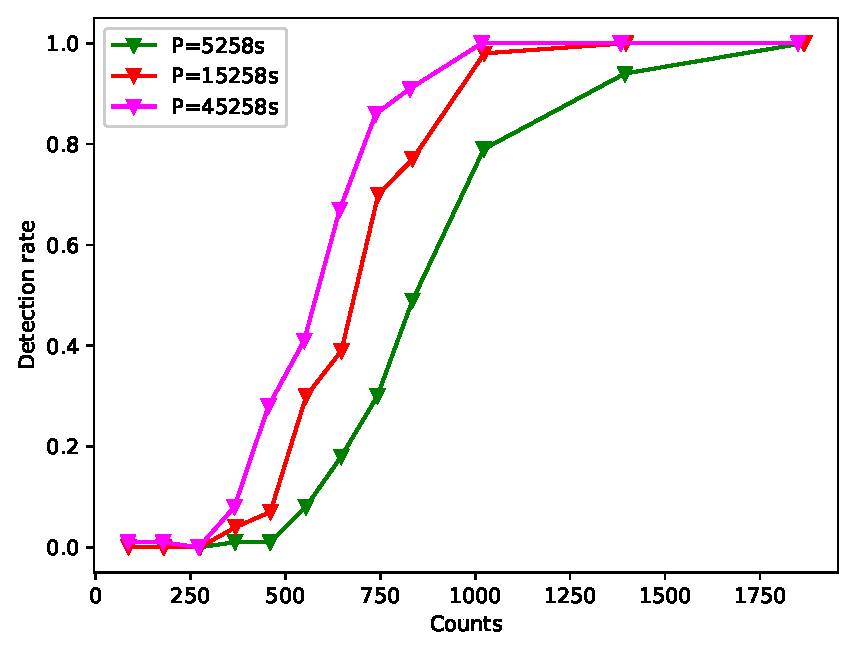
\includegraphics[scale=0.61]{./figure/sim_LW/eclipse_cut.eps}
\caption{Detection rate obtained from simulation results for eclipsing models. Magenta, red and green denotes for P=45258s, 15258s and 5258s respectively. }\label{fig:eclipse}
\end{figure}

We have also run simulations to estimate the rate of false detection, which refers to the detection of a periodic signal from a constant light curve. We use a sinusoidal light curve with $P$=5 yr and $A_0$=0.5 to approximate a constant flux with slight variation, finding no detection of periodic signals at any given values of total counts from 50 to 5000. 
Therefore it seems safe to conclude that the false detection rate is essentially zero for the GL algorithm applied to the LW data. 

\section{Period Searching Results}\label{sec:results}
%\subsection{Filtering detections}
According to the simulations in Section~\ref{subsec:simulation}, a periodic signal is hard to detect in sources with total counts $C\lesssim$100, even in the case of high variation amplitudes.  
Therefore, we restrict our period searching to sources with $C \geq 100$, which include 667 of the 847 sources in the raw list.

Adopting a probability threshold of 90\%, we obtain 48 tentative periodic signals from the three period ranges. However, it is necessary to filter spurious detections, which may be caused by several effects:

(i) By design, the ACIS is dithered to distribute photons over more CCD pixels to avoid pile-up and to fill CCD gaps. The dither period is 706.96 s in pitch and 999.96 s in yaw. Any signal detected at these two periods and their harmonics are thus excluded. These are mostly found in sources located close to CCD gaps, where dithering significantly reduces the number of detected source in a periodic fashion. 
A related concern is how dithering would affect the detection of genuine periods.  
We run simulations to test this effect. Specifically, we generate simulated sinusoidal light curves with $P$ = 5072.97 sec and $C$ = 293. 
This choice is motivated by one particular periodic source (\#5 in Table~\ref{tab:src}), which has a fractional detector coverage of 0.74 (in other words, 26\% of the intrinsic flux is lost due to dithering into the CCD gap), the lowest among all detected periodic sources. The dithering effect is mimicked by artificially removing the simulated counts according to a probability distribution calculated by the CIAO tool \emph{dither\_region}. 
No difference is found in the resultant detection rate, compared to that without dithering. 
%Out of concern about the dither effect on period searching, we compute the fractional area covered by chips (hereafter FA) for each source in each observation. FA equals 1 when source region are not affected by gaps. After, weighting the FA in total exposure time, we define $\overline{FA}$ for each source. Most of $\overline{FA}$ are beyond 0.9, except for \#5, which is 0.74. Thus we run 100 simulation for this source in two cases. One for no dithering and the other for dithering. It turns out no difference in detection rate. In general, we can neglect the dither effect. 

(ii) In certain sources, multiple detections can be caused by second and third harmonics of the same intrinsic signal (i.e., 2 and 3 times the true period). These can be easily identified by the sign of double-peak or triple-peak in the phase-folded light curve, provided that the intrinsic signal has a single-peak structure. However, the intrinsic structure might be double-peak, and in such cases it is more difficult to distinguish the true period and the half harmonics (i.e., half the true period). Hence we assume that there is no half harmonics and always take the lowest period among the multiple detections as the true period. This is consistent with the outcome of our simulations (Section~\ref{subsec:simulation}). Appendix~\ref{harmonics} provides more discussions about harmonics.

(iii) Strong flux variations or outbursts occupying one particular observation can also cause a false periodic signature. This is because the GL algorithm, which analyzes the phase-folded light curve, can be fooled if there were too many photons found in a single observation, producing excess in certain phase bins. In this case the algorithm may "think" there exists a period especially in the third period range. Among the sources with tentative periods, four exhibit a variability index VI$>10$, indicating strong variations. We thus reanalyze their light curves from two subsets of observations: (i) those covering only the outburst and (ii) those excluding the outburst. For three of them, the tentative period cannot be recovered in either subset. Therefore, these three signals are probably false detections. The remaining source is kept since its period can be recovered in both the outbursting and quiescent epochs.

%\subsection{Confirmed Periods}
The above filtering thus results in 25 valid periodic signals in 23 sources.
Among them, 10 periodic signals were reported by \citet{2012ApJ...746..165H} and are confirmed here with the GL algorithm, while the remaining 15 periods are new discoveries (a comparison between our work and \citealp{2012ApJ...746..165H} is addressed in Section~\ref{subsec:compare}). 
The basic information of these periodic sources are listed in Table~\ref{tab:src}, sorted by the order of increasing period. 
The source locations are marked in Figure~\ref{fig:FoV}.

Two sources each exhibit two different periods, hence we have assigned each of them two IDs: \#1/\#14 and \#21/\#22.  
The phase-folded light curves at the two modulation periods are shown for source \#1/\#14 in the upper panels of  Figure~\ref{fig:pCV_sample_1} and for source \#21/\#22 in the upper panels of Figure~\ref{fig:pCV_sample_2}. 
The number of phase bins, between 20 to 50, is chosen to optimally display substructures in the light curve. 
While the GL algorithm does not rely on quantifying the local background, for comparison we plot in these panels the estimated background level (yellow strip, the width of which represents 1\,$\sigma$ Poisson error; Section~\ref{subsec:detect}).
 
For source \#1, the width in phase with flux lower than average is about 0.5, longer than the value for \#14, which is about 0.3. This difference holds out the view that the short period caused by rotation with the alternation of accretion column.
While for source \#21, the weak variation indicates the rotation modulation. And the apparent sharp, narrow eclipsing in \#22 strongly sustain that the orbit modulation with high inclination angle. Considering that the angle between magnetic axis and rotation axis is usually small, it also support for the weak variation of spin modulation.
The characteristics of the phase-folded light curves provide important clues to the source origin, which will be further addressed in Section~\ref{subsec:class}.

The phase-folded light curves are complemented by the long-term, inter-observation light curve, shown in the lower left panel of Figures~\ref{fig:pCV_sample_1} and \ref{fig:pCV_sample_2}, 
and by the source spectrum (see Section~\ref{sec:spectra}),
shown in the lower right panel of Figures~\ref{fig:pCV_sample_1} and \ref{fig:pCV_sample_2}. 
%For middle panel, the valid detection (defined in \ref{subsec:detect}) are plotted with dots plus error range. While the non-valid detection are shown in arrows, providing only the upper limits. Meanwhile, the x-axis in right panel were plotted in discontinuous style for better demonstration effect, since the short interval over the last eight observations. 
%For right panel, the spectra illustrated here were fitted in the range of 1--8 keV, consistent with the timing analysis. 
Similar figures of the remaining 21 sources are presented in Appendix~\ref{appen:fig}.


\begin{table*}
\centering
\begin{threeparttable}
\caption{Information on the periodic X-ray sources in the Limiting Window \label{tab:src}}
\begin{tabular}{lccccccccccc}
\hline
\hline
ID& R.A. & Decl. & Period & $P_{\rm GL}$ & H-ID & $C$ & $A_0$ & $P_{det}$ & $P_{det}'$ & VI & Harmonics
\\
LW & $\circ$ & $\circ$ & (s) & & & & & \% & \% & & 
\\ 
(1) & (2) & (3) & (4) & (5) & (6) & (7) & (8) & (9) & (10) & (11) & (12)
\\
\hline
1$^\dag$ & 267.77173 &	-29.61332 & 853.83 & 0.90277 &-& 202 & 0.76  & 86 &-& 1.92 &- 
\\
2 & 267.76657 &	-29.57529 & 3820.83 & 0.99222 &-& 902 & 0.54 & 99 &- & 1.94 &-
\\
3 & 267.82829 &	-29.63660 & 4728.90 & 1.00000 & H6 & 394 & 0.75 & 98  & 99 & 2.13 & \text{Third}
\\
4 & 267.94766 &	-29.70427 & 4886.79 & 0.99994 &H8 & 784 & 0.56 & 100 & 98 & 1.90 &- 
\\
5 & 267.86255 &	-29.61859 & 5072.97 & 0.99933 &-& 293 & 0.76 & 100 &-&  2.34 &\text{Second}
\\
6 & 267.84831 &	-29.63212 & 5130.57 & 1.00000 & H2 & 437 & 0.76  & 100 & 100 & 2.51 & \text{Second}
\\
7 & 267.86651 &	-29.58575 & 5144.97 & 0.99880 &-& 335 & 0.77 & 100 &-& 2.48 & \text{Second}
\\
8 & 267.90982 &	-29.55845 & 5158.75 & 1.00000 &-& 121 & 1.00 & 100 &-& 2.30 & \text{Second}
\\
9 & 267.88075 &	-29.48562 & 5231.49 & 0.94949 &-& 347 & 0.67 & 100 &-& 1.65 &-
\\
10 & 267.91616 &	 -29.66900 & 5252.93 & 0.91425 &-& 211 & 0.83 
	& 100 &-&-&-
\\
11 & 267.83116 &	 -29.61651 & 5261.93 & 1.00000 & H10 & 438 & 0.88 & 100 & 31 & 1.46 & \text{Second}
\\
12 & 267.73141 &	 -29.49721 & 5334.76 & 0.99952 &-& 760 & 0.51 
	& 100 &-& 1.25& \text{Second}
\\
13 & 267.96901 &	 -29.58142 & 5501.16 & 0.99094 &-& 512 & 0.61 
	& 100 &-& 2.89 &-
\\
14$^\dag$ & 267.77173 & -29.61332 & 5608.21 & 0.96821 &-& 202 & 0.81 & 100 &-& 1.92& \text{Third}  
\\
15 & 267.89161 &	 -29.46508 & 6335.85 & 1.00000 & H5 & 823 & 0.62  & 100 & 100 & 2.09 & \text{Second} 
\\
16 & 267.89024 &	 -29.55369 & 6597.55 & 1.00000 & H9 & 487 & 0.72  & 100  & 99 & 4.30 & \text{Second}
\\
17 & 267.87162 &	 -29.49011 & 7448.98 & 0.99999 & H3 & 535 & 0.73  & 100  & 100 & 1.76 & \text{Second}
\\
18 & 267.78806 &	 -29.58177 & 7756.19 & 0.99941 &-& 214 & 0.91 & 98 &-& 4.76 &\text{Second}
\\
19 & 267.88203 &	 -29.49922 & 8546.28 & 1.00000 &H4 & 3402 & 0.30  & 99 & 93 & 3.27 & \text{Second}
\\
20 & 267.82785 &	 -29.50770 & 8844.82 & 0.90987 &-& 263 & 0.69 
	& 93 &-& 1.82 & \text{Second}
\\
21$^\ddag$ & 267.96375 & -29.55290 & 9877.52 & 0.99992 & - & 1963 & 0.40 & 100 &-& 1.44&- 
\\
22$^\ddag$ & 267.96375 & -29.55290 & 10342.30 & 1.00000 & H1 & 1963 & 0.76 & 100 & 99 & 1.44 &-
\\
23 & 267.84487 &	 -29.57680 & 12002.70 & 1.00000 & H7 & 307 & 1.00 & 100  & 100 & 1.86 & \text{Second}
\\
24 & 267.83142 &	 -29.65992 & 47317.12 & 0.98850 &- & 138 & 0.88 
	& 87 &-&- &-
\\
\hline
%\hline
F1 & 267.90974 &	-29.71112 & 42219.03 & 1.00000 & - &1039&-  &-&-&23.6&-
\\
\hline
\end{tabular}
\begin{tablenotes}
      \small
      \item 
      Notes:
      (1) Source sequence number assigned in the order of increasing period. The same source with multiple period signal was denoted as \dag and \ddag. F1 represents the periodic foreground source.
(2) R.A.(J2000) of the centroid of source. 
(3) Decl.(J2000) of the centroid of source. 
(4) The modulation period determined by GL method.
(5) The probability of periodic signal defined by Eqn.~\ref{A20}. 
(6) The cross-match results with previous work. $H_{i}$ represents the $i$th source in Table 2 of \cite{2012ApJ...746..165H}. 
(7) The number of counts in the 1-8 keV band. 
(8) The amplitude of variation obtained in this work. 
(9) The detection probability of periodicity based on simulations of 100 sinusoidal light curves for each source.
(10) The detection probability of periodicity simulated as the same process described in column(9), while the amplitude are taken from \cite{2012ApJ...746..165H}.
(11) $\rm VI=S_{max}/S_{min}$, where $\rm S_{max}$ and $\rm S_{min}$ are the maximum and minimum photon fluxes among all the valid detections. For source \#10 and \#24, no VI are provided since the lack of valid detections.
(12) The note gives the significant harmonic detected by the algorithm.
    \end{tablenotes}
\end{threeparttable}
\end{table*}

\begin{figure*}
\begin{minipage}[b]{0.45\textwidth}
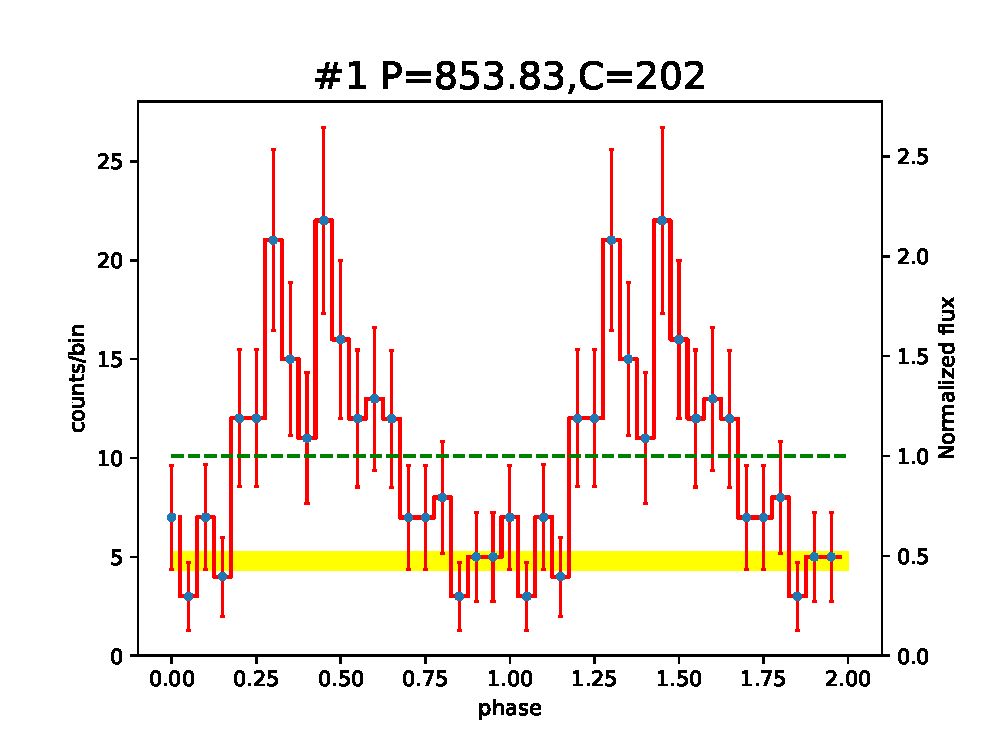
\includegraphics[width=\textwidth]{./figure/LW/pfold_lc_324001.eps}
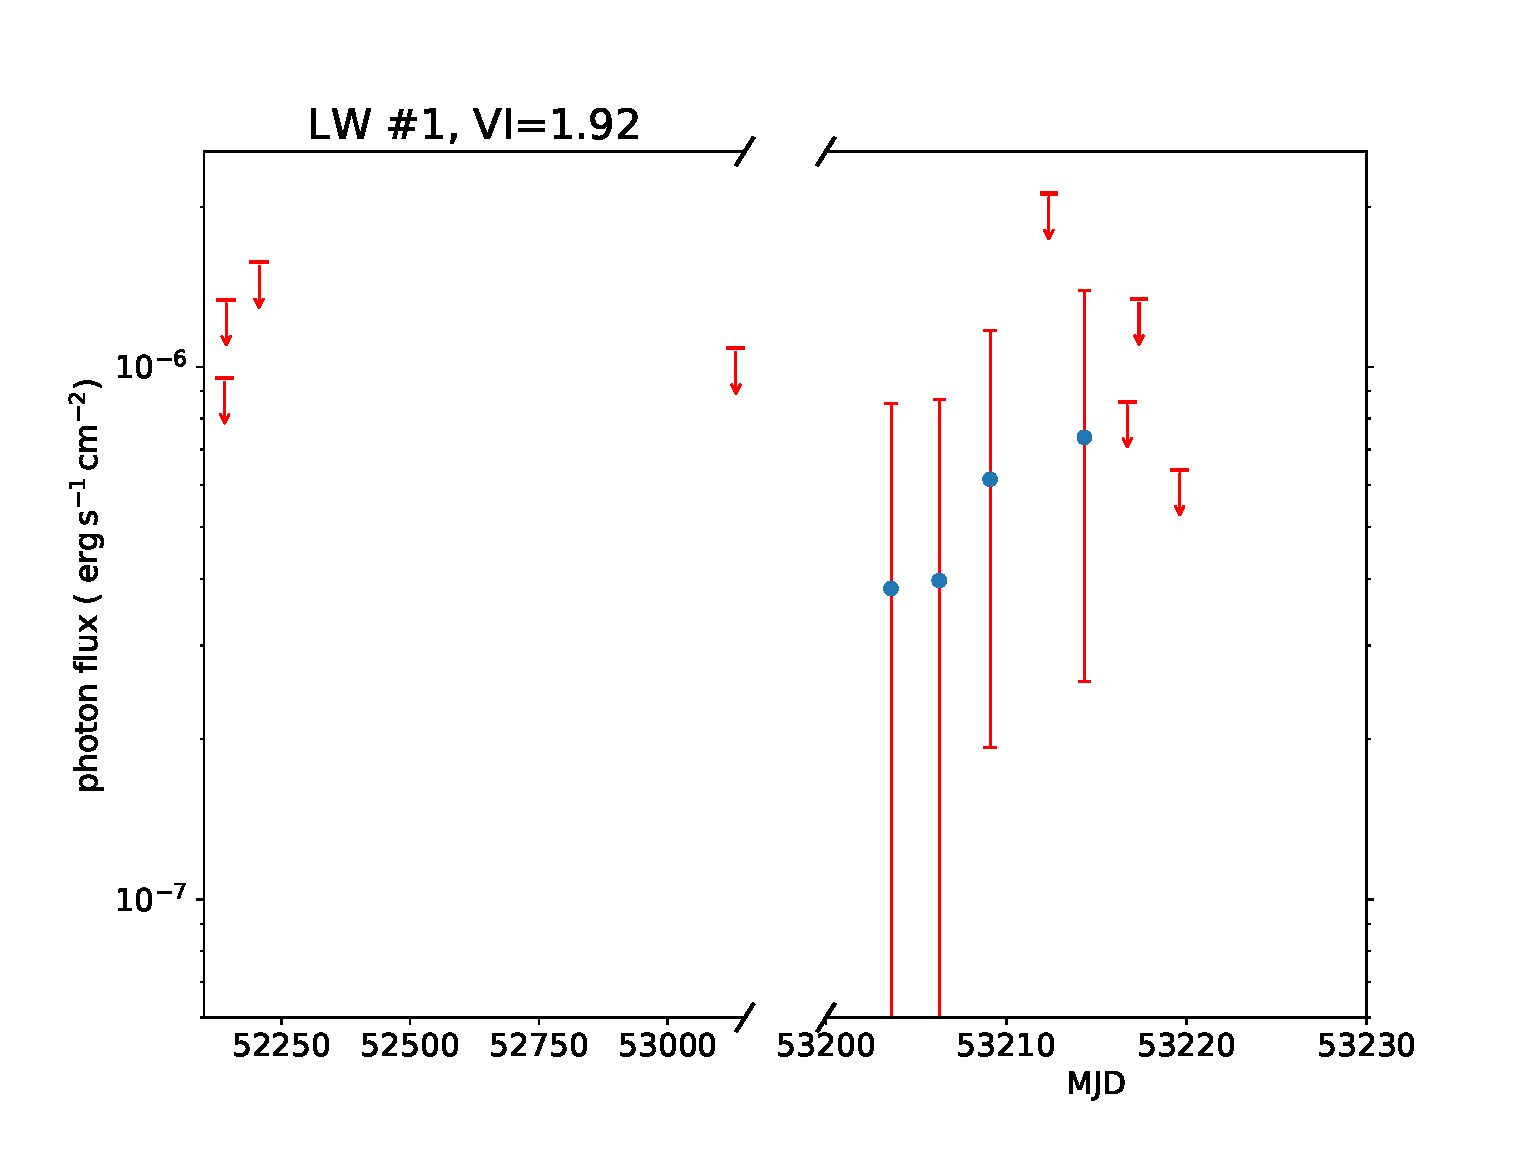
\includegraphics[width=\textwidth]{./figure/LW/324001_lc.eps}
\end{minipage}
\begin{minipage}[b]{0.45\textwidth}
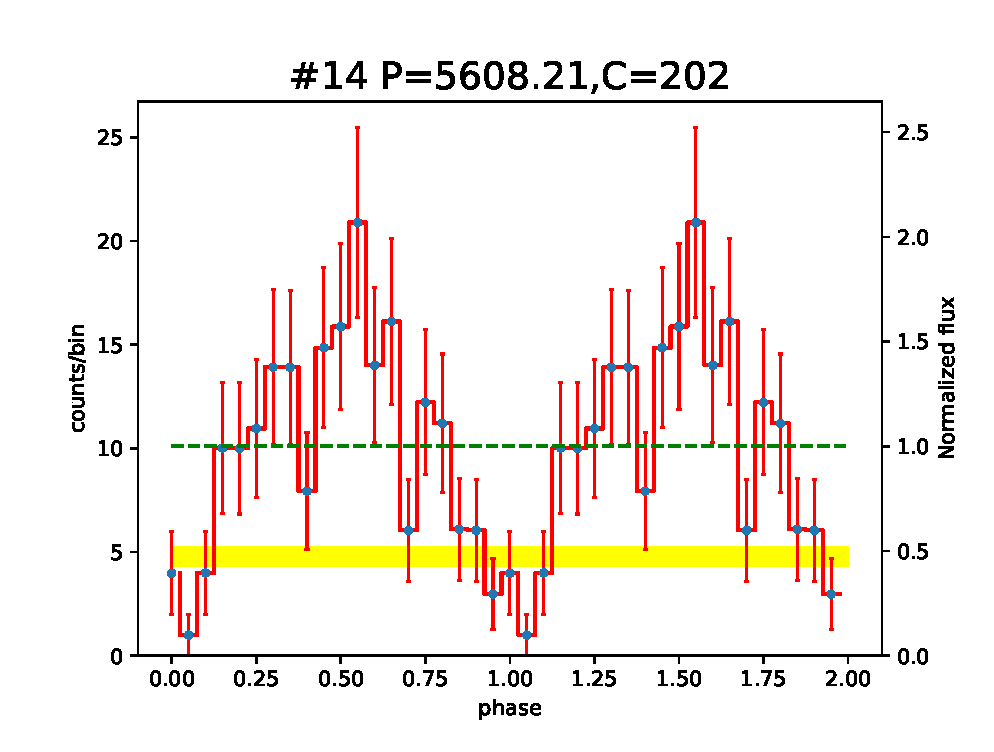
\includegraphics[width=\textwidth]{./figure/LW/pfold_lc_324002.eps}
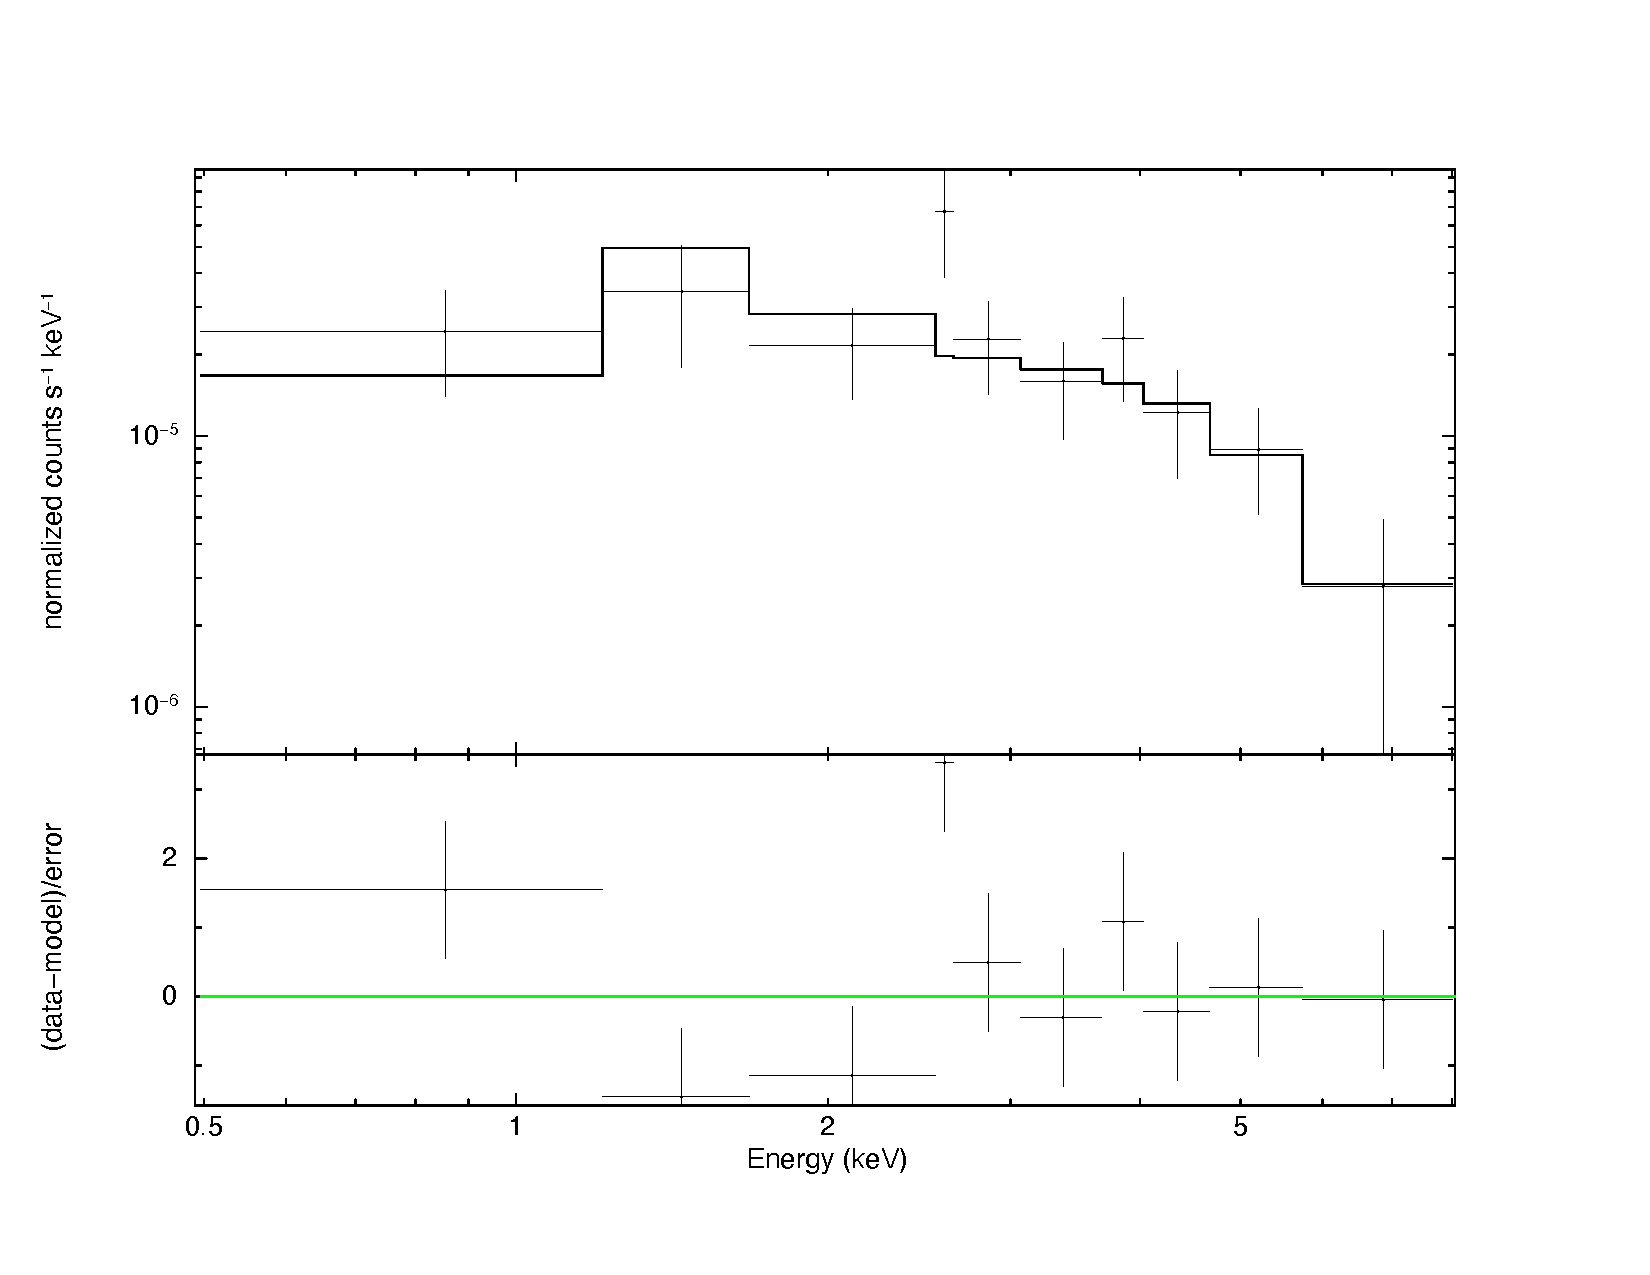
\includegraphics[width=1.0\textwidth]{./figure/LW/324001_spec.pdf}
\end{minipage}
\caption{The phase-folded light curve at the two modulation periods (up), the long-term, inter-observation light curve (lower left) and the spectra (lower right) for \#1(\#14) source.
For upper right panel, the valid detection (defined in Section~\ref{subsec:detect}) are plotted with dots plus error range. While the non-valid detection are shown in arrows, providing only the upper limits. Meanwhile, the x-axis in right panel were plotted in discontinuous style for better demonstration effect, since the short interval over the last eight observations.
For lower right panel, the spectrum are plotted over 1-8 keV to keep the same range with timing analysis.
}
\label{fig:pCV_sample_1}
\end{figure*}

\begin{figure*}
\begin{minipage}[b]{0.45\textwidth}
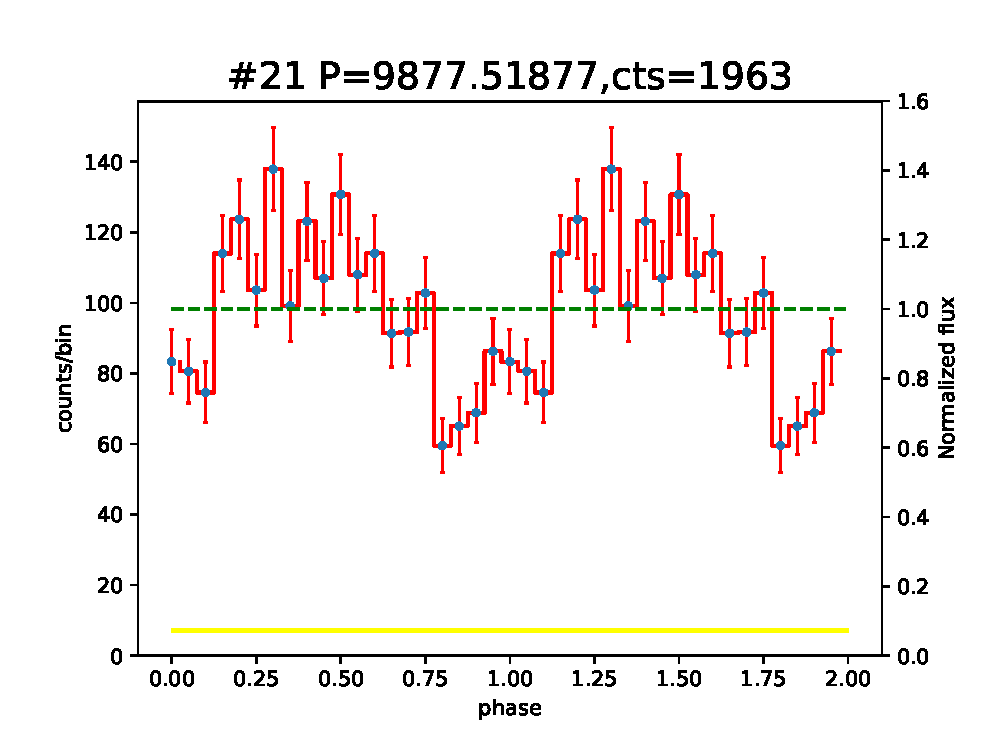
\includegraphics[width=\textwidth]{./figure/LW/pfold_lc_153001.eps}
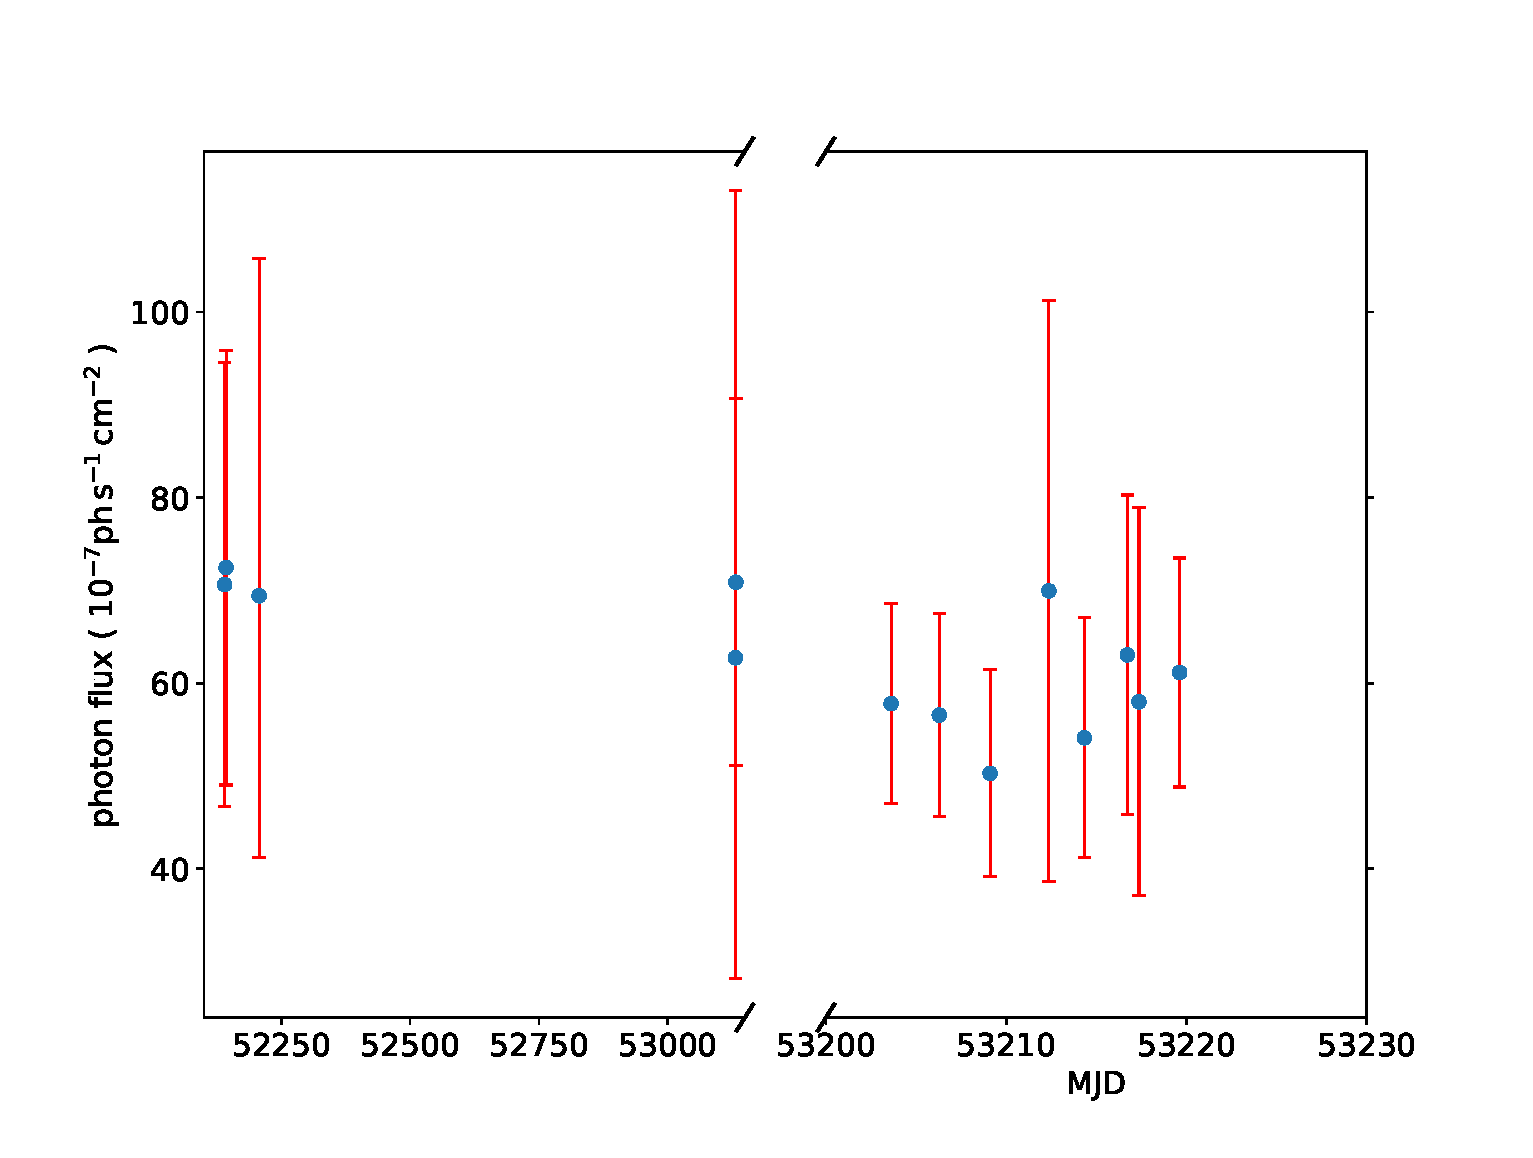
\includegraphics[width=\textwidth]{./figure/LW/153001_lc.eps}
\end{minipage}
\begin{minipage}[b]{0.45\textwidth}
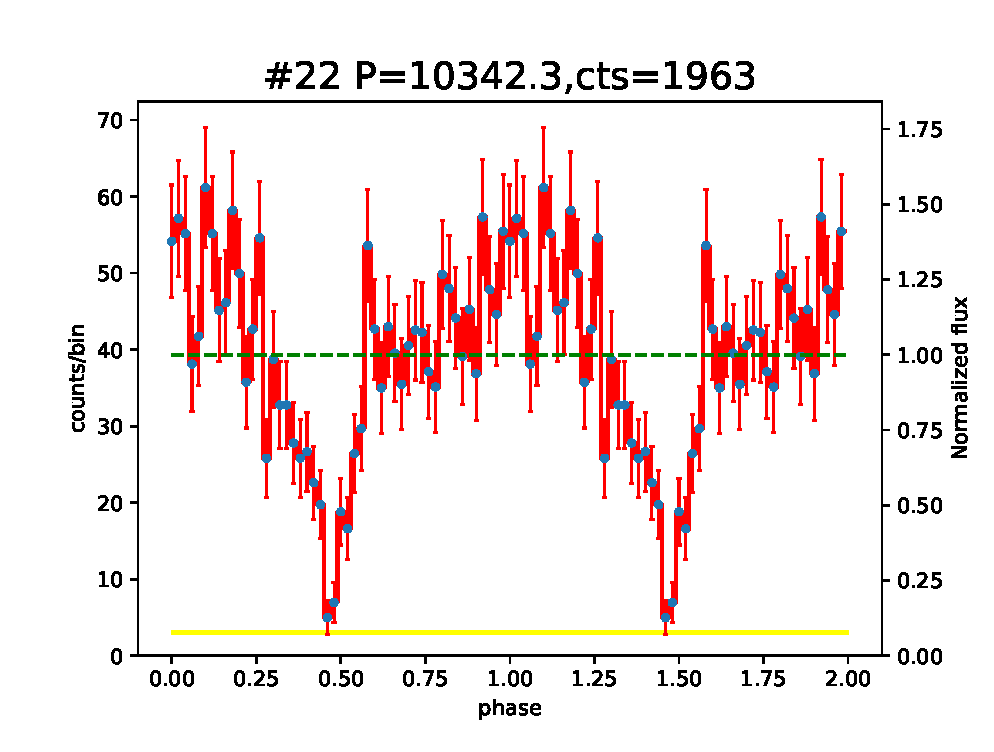
\includegraphics[width=\textwidth]{./figure/LW/pfold_lc_153002.eps}
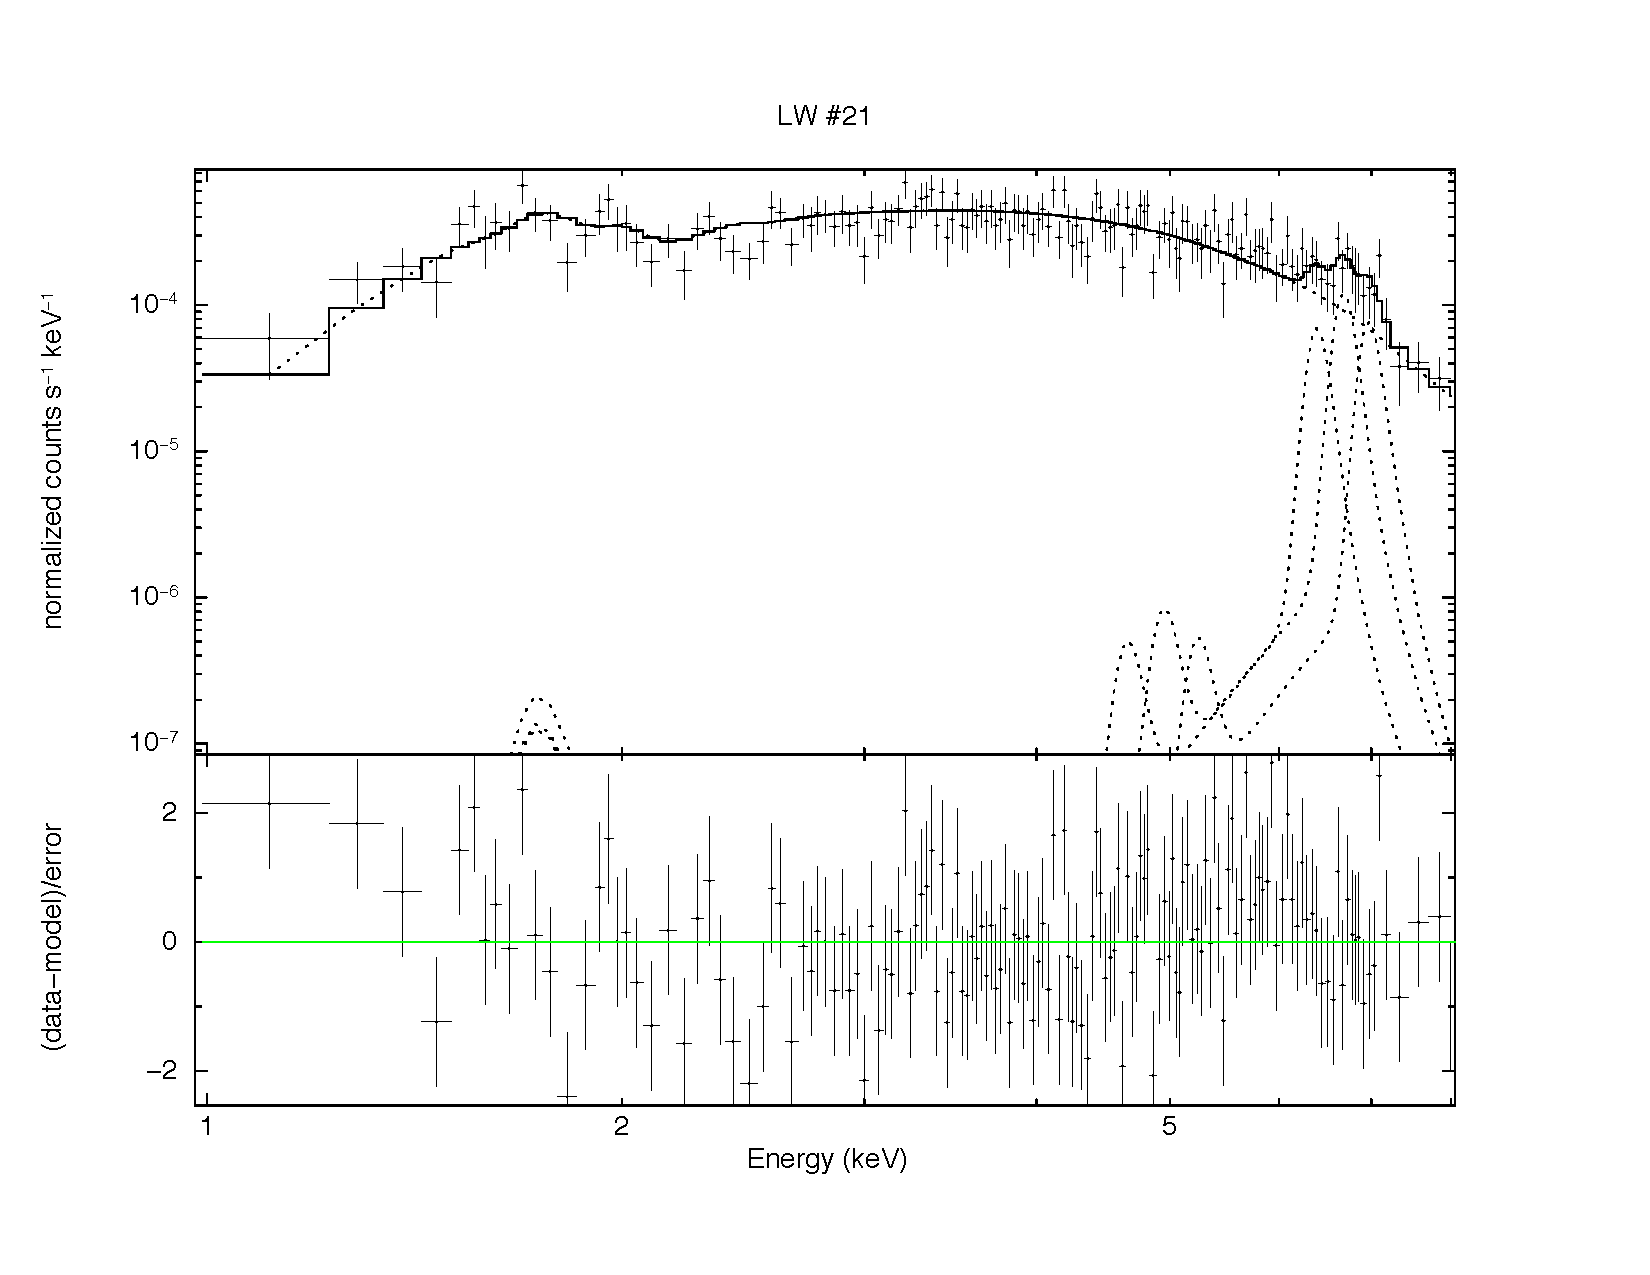
\includegraphics[width=1.0\textwidth]{./figure/LW/153001_spec.pdf}
\end{minipage}
\caption{Similar to Figure~\ref{fig:pCV_sample_1}, but for source \#21/\#22.}
\label{fig:pCV_sample_2}
\end{figure*}

\section{X-ray spectral analysis}\label{sec:spectra}
We perform spectral analysis for all 23 confirmed periodic sources to gain insight on their nature. Source and background spectra are extracted from the same regions as described in Section~\ref{subsec:detect}, along with the ancillary response files (ARFs) and redistribution matrix files (RMFs), by using the CIAO tool \emph{specextract}. 
The spectra from individual observations are then coadded to form a combined spectrum of a given source, with the corresponding ARFs and RMFs weighted by the effective exposure. 
Further, the spectrum is adaptively binned to achieve a minimum of 20 counts and a signal-to-noise ratio greater than 2 per bin.

The resultant spectra are analyzed using XSPEC v12.9.1.
%The reason we present the fitting results of 0.5-8 keV here is to constrain the absorption. Notice that the choice of energy range is not consistent with the illustration of spectra in Figure \ref{fig:Figure_p}, even though it has little impact on exhibition. 
Since these sources are expected to be CVs, we adopt a fiducial spectral model \citep{2018ApJS..235...26Z,2019ApJ...882..164X}, which consists of a bremsstrahlung continuum and three Gaussian lines centered at 6.40, 6.68 and 6.97 keV, all these components subject to an unknown line-of-sight absorption (\emph{phabs} in XSPEC). 
The three lines (hereafter referred to as the 6.4, 6.7 and 7.0 keV lines) correspond to neutral Fe K$\alpha$, Fe\,XXV K$\alpha$ and Fe\,XXVI Ly$\alpha$, respectively, which are among the most commonly detected emission lines in CV spectra. The latter two lines, in particular, arise from the post-shock plasma near the WD surface, and their flux ratio ($I_{7.0}/I_{6.7}$) has proven to be a robust tracer of the plasma temperature, hence also a good indicator of the WD mass \citep{2016ApJ...818..136X}.

It turns out that the plasma temperature ($T_{\rm b}$) is not well constrained in most sources, due to a moderate number of counts and the insufficient sensitivity of {\it Chandra} at energies above 8 keV. Hence for such cases we fix $T_{\rm b}$ at 40 keV, which is typical of IPs when their hard X-ray (up to tens of keV) spectra are available \citep{2016ApJ...818..136X,2016ApJ...826..160H}.
Setting a lower value of $T_{\rm b}$, for instance, at 20 keV, does not affect our following conclusions. 

%The flux ratio of Fe XXVI to Fe XXV emission lines (hereafter $I_{7.0}/I_{6.7}$) could be interrelated to the $M_{WD}$ by uniting the $I_{7.0}/I_{6.7}$-$T_{max}$ and $T_{max}-M_{WD}$ relations \citep{2019ApJ...882..164X}. 
Again due to the limited number of counts, most of the periodic sources show weak or non-detected Fe lines.  
We have applied a bootstrapping method using the {\it multifake} tool in XSPEC to derive the 90\% confidence range for the fluxes of the three Fe lines. It turns out that only one sources, \#21 (same as \#22), shows a significant line at both 6.7 keV and 7.0 keV.  
The flux ratio and its 90\% error are similarly determined for this sources, resulting in $I_{7.0}/I_{6.7} = 0.91^{+1.22}_{-0.56}$ for \#21.   
%The value of flux ratios are presented together with their 68.3\% confidence range (see column (4) and (5) in Table \ref{tab:spec}). 
According to the empirical line ratio--WD mass  ($I_{7.0}/I_{6.7}$--$M_{\rm WD}$) relation of \citet{2019ApJ...882..164X}, which is calibrated with CVs in the solar neighborhood, we can infer $M_{\rm WD} \approx 0.8 \, (1.2) $  $M_\odot$ for \#21, provided that both sources are IPs (DNe). 
It is noteworthy that there exists no empirical $I_{7.0}/I_{6.7}$--$M_{\rm WD}$ relation for polars, mainly due to the small number of known polars in the solar neighborhood \citep{2019ApJ...882..164X}. 

Based on their best-fit results, the source with $N_H$ lower than $5 \times 10^{21} cm ^{-2}$ are considered as foreground source.
We further divide the 22 periodic sources into two groups based on their luminosities. Here source F1 is excluded since we are only interested in sources located in the bulge. The H (L) group consists of 6 (16) sources having an unabsorbed 1--8 keV luminosity above (below) $\rm 1.0\times10^{32}~erg ~s^{-1}$, which is derived from the individual best-fit spectral model. 
The cumulative spectrum of each group is fitted with the same fiducial model, i.e., bremsstrahlung plus three Gaussian lines. The improved S/N in the cumulative spectrum allows us to detect all three Fe lines and constrain their flux ratios.  
%And the best-fit results are presented in Table \ref{tab:spec}. 
%The H and L spectra are shown in Figure \ref{fig:pCV_spec} over the energy range of 0.5-8 keV. 
%Using the XSPEC tool \emph{multifake}, we have gotten well constrained line ratios for this two subtypes. 
The group has $I_{7.0}/I_{6.7} = 0.78^{+0.18}_{-0.16}$, thus inferring a mean WD mass of $M_{\rm WD} \approx 0.8$ (1.2) $M_\odot$ if they are IPs (DNe). 
On the other hand, the L group shows no constrain of line ratio, we can only provide its upper limit, i.e., 0.39, corresponding $M_{\rm WD} < 0.45$ (0.80) $M_\odot$ if they are IPs (DNe). 

Results of the above spectral analysis are summarized in Table \ref{tab:spec}.
\begin{table*}
\centering
\begin{threeparttable}
\caption{X-ray spectral properties of the periodic sources \label{tab:spec}}
\begin{spacing}{1.19}

\begin{tabular}{lccccccc}
\hline
\hline
ID & $N_{\rm H}$ & $T_{\rm b}$ & $I_{6.4}/I_{6.7}$ &
$I_{7.0}/I_{6.7}$ &  $I_{6.7}$ & $\chi^2/dof$ & $L_{\rm 1-8}$ 
\\
(1) & (2) & (3) & (4) & (5) & (6) & (7) & (8)
\\
LW & $10^{22}\rm~cm^{-2}$ & keV & & & $10^{-8}\rm~ph~cm^{-2}~s^{-1}$ & & $10^{31}\rm~erg~s^{-1}$ 
\\
\hline

1$^\dag$ & $0.51^{+0.75}_{-0.34}$ & 40 (fixed)  &-&-&-& 1.14/5  & $1.82^{+0.64}_{-0.51}$
\\
2 & $2.17^{+0.54}_{-0.46}$ & $20.7^{+56.9}_{-9.92}$ &-&-&-& 0.86/78  & $23.1^{+2.70}_{-2.01}$
\\
3 & $1.34^{+0.70}_{-0.40}$ & $46.4^{+46.1}_{-38.5}$ &-&-&-& 0.98/33  & $6.61^{+1.05}_{-0.77}$
\\
4 & $1.15^{+0.69}_{-0.50}$ & $11.3^{+53.3}_{-4.71}$ &-&-&-& 0.91/27  & $22.5^{+2.94}_{-4.42}$
\\
5 & $1.02^{+0.27}_{-0.23}$ & 40 (fixed) &-&-&-& 1.00/33 &  $5.59^{+0.77}_{-0.70}$
\\
6 & $1.82^{+0.57}_{-0.50}$ & $6.90^{+12.4}_{-2.90}$ 
	&-&-&-& 1.12/42 &  $9.23^{+1.24}_{-1.11}$
\\
7 & $1.62^{+0.62}_{-0.49}$ & $41.6^{+43.0}_{-32.3}$ &-&-&-& 0.86/39 &  $6.70^{+0.89}_{-0.81}$
\\
8 & $2.06^{+1.51}_{-0.94}$ & 40 (fixed) &-&-&-& 0.93/7 &  $1.76^{+0.54}_{-0.42}$
\\
9 & $1.29^{+1.34}_{-0.67}$ & $20.8^{+95.8}_{-20.8}$ &-&-&-& 1.10/7 &  $3.50^{+1.22}_{-0.86}$
\\
10 & $2.50^{+7.25}_{-1.56}$ & 40 (fixed)  &-&-&-& 0.85/5 &  $2.14^{+1.76}_{-0.75}$
\\
11 & $1.85^{+0.39}_{-0.33}$ & 40 (fixed)  &-&-&-& 1.22/47 &  $9.49^{+1.11}_{-1.02}$
\\
12 & $6.23^{+9.67}_{-3.66}$ & 40 (fixed) &-&-&-& 0.78/6 &  $7.58^{+5.76}_{-2.93}$
\\
13 & $0.90^{+0.30}_{-0.24}$ & 40 (fixed) &-&-&-& 1.15/38 &  $8.48^{+1.12}_{-1.04}$
\\
14$^\dag$ & $0.51^{+0.75}_{-0.34}$ & 40 (fixed) &-&-&-&  1.14/5 &  $1.82^{+0.64}_{-0.51}$
\\
15 & $1.46^{+0.48}_{-0.38}$ & 40 (fixed) &-&-&-&  1.16/42 & $12.8^{+1.77}_{-1.61}$
\\
16 & $0.89^{+0.18}_{-0.16}$ & 40 (fixed) &-&-&-&  1.43/51  & $8.47^{+0.88}_{-0.83}$
\\
17 & $2.68^{+0.63}_{-0.52}$ & 40 (fixed)  &-&-&-&  0.75/36 & $11.3^{+1.61}_{-1.45}$
\\
18 & $2.01^{+0.92}_{-0.66}$ & 40 (fixed)  &-&-&-&  0.53/14  & $4.21^{+0.89}_{-0.77}$
\\
19 & $1.82^{+0.10}_{-0.10}$ & 40 (fixed)  &-&-&-& 0.95/185  & $83.9^{+3.25}_{-3.16}$
\\
20 & $2.09^{+2.45}_{-1.16}$ & $4.04^{+28.2}_{-2.54}$ &-&-&-& 1.04/12  & $5.39^{+1.81}_{-1.47}$
\\
21$^\ddag$ & $2.83^{+0.25}_{-0.23}$ & 40 (fixed)  & $0.47^{+0.72}_{-0.35}$ & $0.91^{+1.22}_{-0.56}$ & 31.7 & 1.10/147  & $60.00^{+3.25}_{-3.12}$
\\
22$^\ddag$ & $2.83^{+0.25}_{-0.23}$ & 40 (fixed)  & $0.47^{+0.72}_{-0.35}$ & $0.91^{+1.22}_{-0.56}$ &  31.7 & 1.10/147  & $60.00^{+3.25}_{-3.12}$
\\
23 & $1.83^{+0.44}_{-0.37}$ & 40 (fixed)  & - &-& - & 1.47/35  & $9.23^{+1.22}_{-1.13}$
\\
24 & $0.83^{+3.31}_{-0.83}$ & $2.30^{+1.59}_{-0.85}$ &-&-&-&  0.80/2 & $0.75^{+0.30}_{-0.28}$ 
\\
\hline
F1 & $0.35^{+0.16}_{-0.13}$ & $4.78^{+3.55}_{-1.58}$ &-&-&-& 1.19/55  & - \\
%$8.73^{+1.09}_{-0.98}$
\hline
H & $1.99^{+0.10}_{-0.97}$ & 40 (fixed)  &  $0.28^{+0.10}_{-0.09}$ & $0.78^{+0.18}_{-0.16}$  & $8.76^{+3.57}_{-3.57}$ & 1.19/205 & $31.8^{+0.95}_{-0.95}	$
\\
L & $1.33^{+0.12}_{-0.11}$ & 40 (fixed)  & $<0.18$  & $<0.39$ & $2.53^{+1.10}_{-1.10}$ & 1.09/168 & $5.36^{+0.24}_{-0.24}$ \\
\hline
\end{tabular}
\end{spacing}
\begin{tablenotes}
      \small
      \item
      Notes: 
      (1) Source sequence number as in Table~\ref{tab:src}, except ``H'' and ``L'', which refer to the bright and faint group of sources (excluding source F1), i.e., having 1--8 keV luminosity above (below) $10^{32}\rm~erg~s^{-1}$. {\dag}Sources 1 and 14 are the same source with two different periods; {\ddag}Sources 21 and 22 are the same source with two different periods. 
(2) Line-of-sight absorption column density.
(3) The bremsstrahlung temperature, in units of keV. Fixed at a value of 40 keV when the spectrum provides no signficant constraint to this parameter.
 (4)-(5) Flux ratio of the 6.4 or 7.0 keV line to the 6.7 keV line.
 (6) Integrated flux of the 6.7 keV line.
 (7) $\chi^2$ and degree of freedom of the best-fit model.
 (8) 1--8 keV unabsorbed luminosity. Quoted errors are at the 90\% confidence level.
\end{tablenotes} 
\end{threeparttable}
\end{table*} 
 
%\end{deluxetable*}
%

%\begin{figure*}[!htbp]
%\centering
%\rotatebox[origin=c,x=11pt,y=146pt]{270}{\includegraphics[width = 0.6\textwidth]{./figure/LW/pCV_brem.eps}}
%\caption{Cumulative spectra with the best-fit model($phabs\times (bremsstrahlung+gaussian+gaussian+gaussian) $).
%The spectrum for H, L set of periodic sources are plotted in red and black respectively. %\label{fig:pCV_spec}}
%\end{figure*}

\section{Discussion}\label{sec:discussion}
\subsection{Comparison with previous work} \label{subsec:compare}
We have detected 25 periodic signals from 23 sources in the LW (Table~\ref{tab:src}). 
In particular, our detections fully recover the 10 periodic signals from 10 sources found by  \cite{2012ApJ...746..165H}, while the remaining 15 periods are new detections. 
Since \cite{2012ApJ...746..165H} and this work have used the same set of {\it Chandra} observations, 
this difference must be owing to the different period searching methods employed.

\cite{2012ApJ...746..165H} employed the LS periodogram,
%extracted only the several nearby observations, all the observations were applied here for timing analysis. That difference was caused by the mechanisms of methods. 
which, as described in Section~\ref{subsec:GL}, handles the photometric light curve, while the GL algorithm processes the phase-folded light curve with tolerance for observing gaps. We have applied the LS periodogram to our data in essentially the same way as \cite{2012ApJ...746..165H} and confirmed that only those 10 periods found in their work can be detected by this method.  The other 15 periods do not result in a significant detection in the LS periodogram, mainly due to the poor efficiency of that algorithm. 
The detection rate is about zero when net counts down to 100 and could not exceed 20\% as net counts climbing to 150, based on the simulation in \cite{2012ApJ...746..165H}.


Besides, we also did 100 times of simulations for each signal. We had to use sinusoidal variations for simulating process though many of them may deviate much from real shape. The counts rate and period can be directly attained from data, while the amplitude is hard to determine since the deviation. In \citet{2012ApJ...746..165H}, they got $A_0$ from $A_{\mathrm{rms}}$ depended on Rayleigh statistics.\citep{1983A&A...128..245B,2003ApJ...599..465M}.
%The definition of $A_{\mathrm{rms}}$ and the relation between 
%$A_{\mathrm{rms}}$ and $A_0$, which were taken by \cite{2012ApJ...746..165H}, are described below.
%\begin{subequations}
%\begin{equation}
%A_{\mathrm{rms}}=\left(\frac{Z_{1}^{2}}{N}\right)^{1 / 2} \frac{N}{N-B}
%\end{equation}
%\begin{equation}
%Z_{1}^{2}=\frac{2}{N}\left\{\left[\Sigma_{j} \cos \phi\left(t_{j}\right)\right]^{2}+\left[\Sigma_{j} \sin ^{2} \phi\left(t_{j}\right)\right]^{2}\right\}
%\end{equation}
%\begin{equation}\label{Arms}
%A_0=\sqrt{2} A_{\mathrm{rms}}
%\end{equation}
%\end{subequations}
%where equation \ref{Arms} only works for sinusoidal modulations. N and B represent the total counts in source region and local background respectively. $t_{j}$ and $\phi\left(t_{j}\right)$ refer to the arrival time and phase of each photon. $Z_{1}^{2}$ is the classical Rayleigh statistic method \citep{1983A&A...128..245B,2003ApJ...599..465M}.
Meanwhile, they provided another way to obtain $A_0$. From phase-folded light curve, they defined $A_{M}={1-R_{min}}/R_{max}$, and $A_{M}=2A_0/({1+A_0})$, where $R_{min}(R_{max})$ is the minimum (maximum) count rate of the folded light curve. 

Though $A_{M}$ depends on the bin size of phase-folded light curve, we still prefer it rather than $A_{rms}$ to get the amplitude, i.e, $A_0$, since the deviation between sinusoidal variation and real shape sometimes made $A_{0}$ exceeds one when it was calculated from $A_{\mathrm{rms}}$. 

Still, we took 90\% as threshold to get valid detection at 0.1\% accuracy. The percentage of valid detection would be represented by $P_{det}$, as shown in column (9) in Table \ref{tab:src}. And $A_{M}$ was obtained with bin size fixed at 20. For directly comparison, we also ran the simulation based on the same $A_{0}$ defined in \citet{2012ApJ...746..165H} for the ten collective sources. A flagrant contrast was illustrated in Figure \ref{fig:com} based on that two columns. Apparently, GL method has better performance compared with LS method.

The improvement on detecting efficiency and data usage brought more periodic signals than \cite{2012ApJ...746..165H}. Additionally, we operated the simulation not only for sinusoidal variation, but also for eclipsing models to describe the dip in orbital modulation. Combining the simulation results and more than twice the sample, we were allowed to discuss the source properties and the distribution of CVs in galactic bulge region on a better level.

\begin{figure}
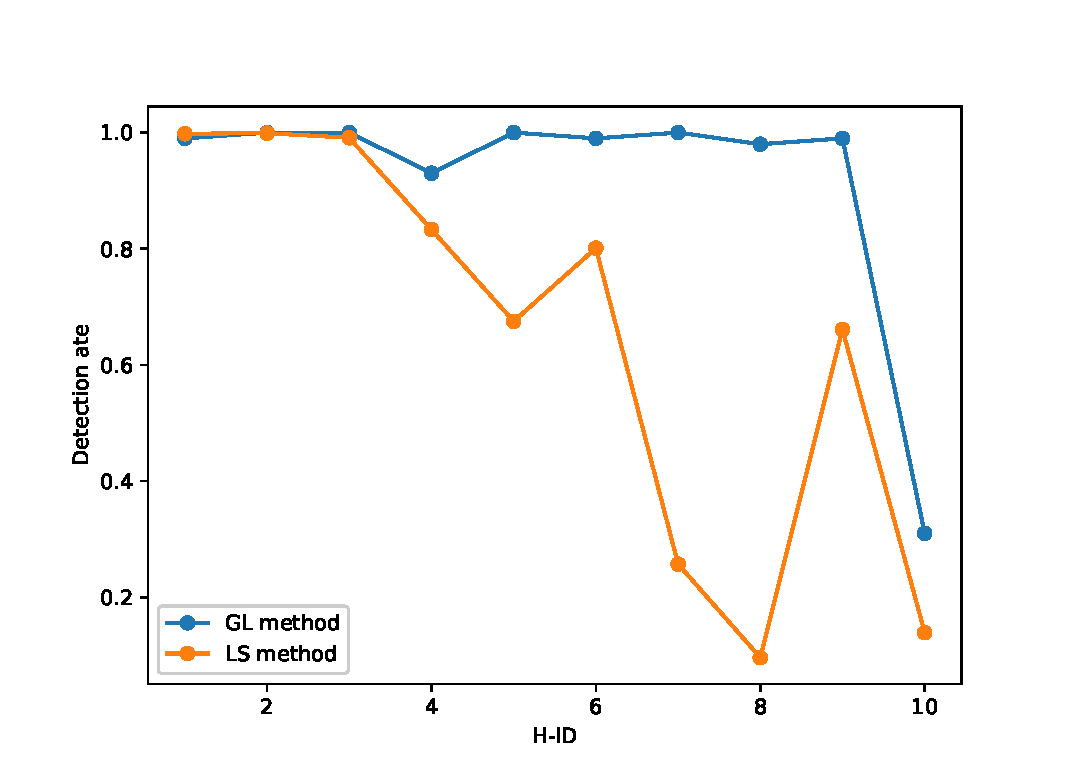
\includegraphics[scale=0.55]{./figure/sim_LW/Pdet_com.eps}
\caption{The comparison of efficiency between two methods. H-ID is the sequence number given by \citep{2012ApJ...746..165H}, same as column(6) in Table \ref{tab:src} \label{fig:com}.The detection rate of LS method are taken from Table 2 in \citep{2012ApJ...746..165H}}.
\end{figure}
\begin{figure}
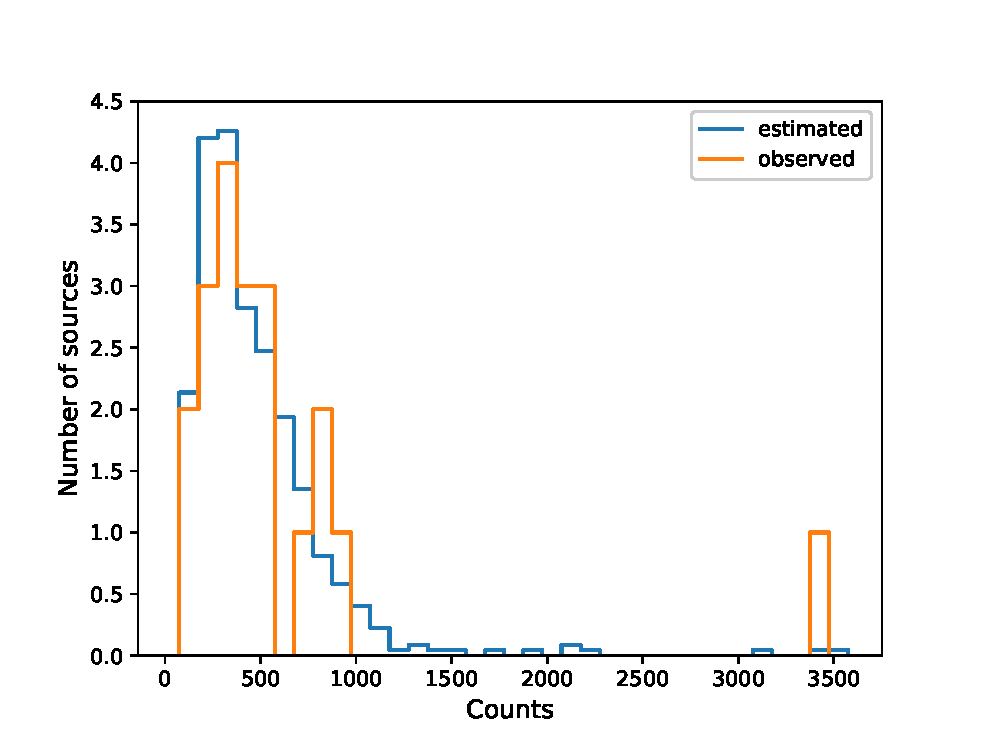
\includegraphics[scale=0.53]{./figure/sim_LW/est_obs.eps}
\caption{The comparison between estimated and the real detected number of sources. \label{fig:NP_sim}}
\end{figure}

\subsection{Classifying the periodic X-ray sources}
\label{subsec:class}
Despite of source F1, whose luminosity can not be estimated for the uncertain distance, 
these periodic sources are with luminosities ranged from $\rm 10^{31}$ to $\rm 10^{33}~erg~s^{-1}$, combined with the period distribution, mostly about 1-3 hours. All of these properties suggest that they belong to cataclysmic variables.
We can barely exclude the probability of these sources being coronally active binaries (ABs), since most ABs are with luminosities lower than $\rm 10^{31}~erg~s^{-1}$ \citep{2006A&A...450..117S}. 

While the case is not applicable for source \#24, with luminosity about $\rm 0.75 \times 10^{31}~erg~s^{-1}$ and plasma temperature about 2 keV. All these features are typical for ABs. Besides, its phase-folded light curve exhibits no emission in half of cycle, indicating the similar radius for two stars. The nearly no emission from one star hinted it could be an A-type star. Then the orbit radius would be around 0.02 AU, taking $3M_\odot$ as the total mass.  

Before we start to discuss the nature of these periodic sources, we should take a look at CVs in the field. Their period distribution, including polars, IPs and DNe, are shown in Figure \ref{fig:N_P}.
It can be easily seen that the period distribution of these LW sources resembles those of polars more than others, since most of these are below the period gap. While DNe and IPs both have a considerable number of systems with period beyond the gap. According to the our simulation results in Section~\ref{subsec:simulation}, this can not be resulted from selection bias of algorithm. 

\begin{figure*}
\centering
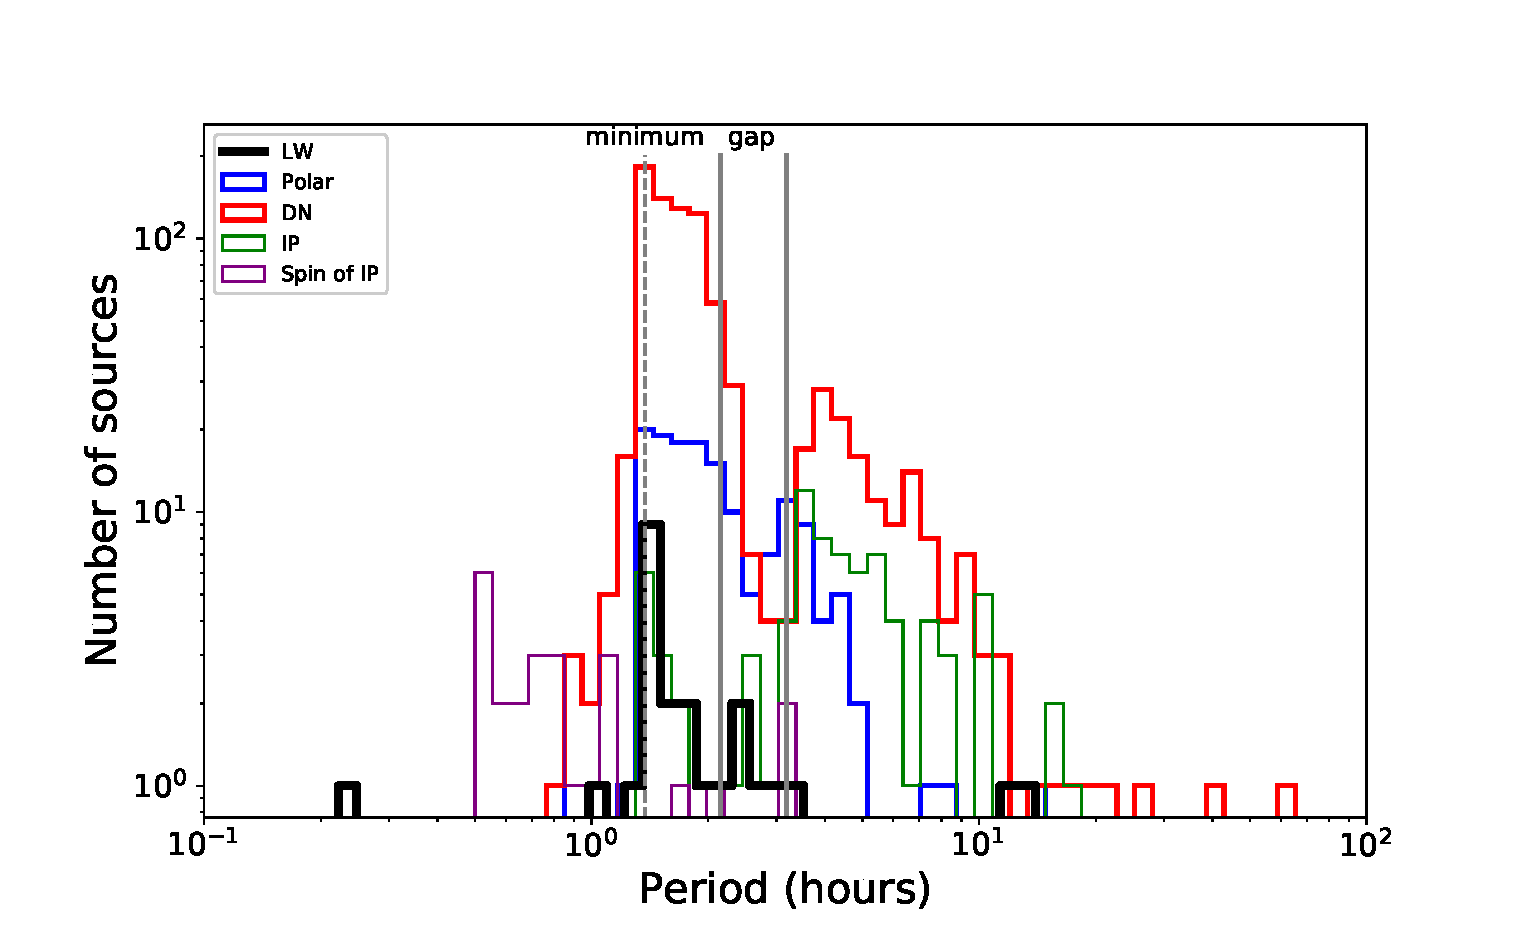
\includegraphics[scale=0.73]{./figure/CV/N_P.eps}
\caption{The period distribution of the LW sources (dark-blue line), the spin (purple) and orbital (green) periods of IPs ,the periods (sky-blue) of polars and the orbital (red) periods of DNe from the RK catalog \citep{2003A&A...404..301R}, version 7.20). The famous period gap(yellow line) and period minimum(orange dashed line) are also plotted, whose value are taken from \citep{2011ApJS..194...28K}.\label{fig:N_P}}
\end{figure*}

For non-magnetic CVs like DNe, the common phase-folded light curve exhibits narrow dip, due to the eclipse of the white dwarf, as modeled in Section~\ref{subsec:simulation}. The typical light curve is like \#22 in Figure \ref{fig:pCV_sample_2}. 	While the simultaneous existence of \#21 and \#22 and the 2\% period difference suggest it might be an asynchronous intermediate polar. Besides, the central dip of \#3, \#18 and \#20 are also similar to this circumstance. Since the eclipse happens in nearly all types of CVs, we could only set three as an upper limit of number of DNe in our sample.

For magnetic CVs, including IPs and polars, their orbit modulation could give rise to more complicated shape of light curve. For polars, consider the simplistic situation, whose accretion is nearly onto one pole, then the shape of light curve would be divided into two groups. Suppose an inclination $i$, the angle between rotation axis and magnetic axis is $\beta$, the magnetic colatitude of accretion is $\epsilon$. Then if $i+\beta+\epsilon > 90^{\circ}$, we would see alternately two poles, the shape would be like \#6, with half of orbit cycle showing no emission. This so-called "two-pole"  behavior are more complicated if the accretion goes to both two poles, the gap with half orbit cycle would be partially filled (like \#16) by second pole's emission or even making the light curve constant. Sometimes it may completely reverse in hard X-ray band cause the accretion shock in second pole producing most of hard X-rays \citep{1985A&A...148L..14H}. On the other hand, if $i+\beta+\epsilon < 90^{\circ}$ and $\beta < i$, in which the accreting pole is always visible , the modulation would caused by the obscuring of accretion stream. The width and depth of the dip in phase space are determined by many reasons and totally unpredictable. 

For IPs, the orbital modulation could be resulted by eclipse of WD, the absorption of X-rays emitted near the white
dwarf surface \citep{1993MNRAS.260..299H}, or the "disc-overflow" model in \citep{1996MNRAS.280..937N}. The shape of light curve in IPs could be any kinds of dips or sinusoidal variation. The only robust identification is to determine both their spin and orbital period, like the \#1(\#14) and \#21(\#22) in our sample.

Based on our current understanding of the shape and distribution of orbital modulation, we conclude that the periodic sources discovered are mostly polars, with several IPs(two determined) and DNe(three as upper limit). 



\subsection{CV populations in the Galactic bulge}
Firstly, we assumed that the fraction of polars in the total sample of 667 sources is $\alpha$. The sinusoidal variation happens in "two-pole" situation, which takes $90^\circ$ in total $180^\circ$. Assuming the fraction of accretion onto one pole is 50\%, then we can set 25\% as the lower limit of fraction for polars with sinusoidal variation intrinsically. We assumed the even distribution for amplitude from 0.5 to 0.9 and took the simulation results for P=5540s and P=45540s as the detection rate for period under(60\% of the total number) and beyond the period gap(40\% of the total number). The value of 60\% and 40\% are estimated from Figure \ref{fig:N_P}. Then we set width=100 for our binning of counts, from 75 to 3575, which consist nearly all detected sources. The choice of value balance the number of counts taken from observation and simulation. 
 The predicted number of periodic sources which "should" be detected in each bin is calculated by:
\begin{equation}
Np_{i}=N_i\times DR \times 25\% \times 667 \times \alpha	
\end{equation}
$N_i$ is the product of number of sources detected in the bin. DR denotes the detection rate weighted from simulation. Then we sum all $Np_{i}$ together and force it equals to 20,  getting $\alpha$ about 16\%. The comparison between $Np_{i}$ and the real detected 20 periodic sources(two determined IPs and one foreground source excluded) are plotted in Figure \ref{fig:NP_sim}. The perfect agreement between their population proves the validity of estimation.

Since the real luminosity function should be gentle than that of  total sample, which means there could be more polars at the bright band, then it demanding lower numbers of polar to balance the high detection rate for bright sources. Besides, with the intrinsic fraction (25\% as the lower limit) increasing, the $\alpha$ decreasing.
In general, the 16\% should be treated as the upper limit for polars, especially when we considered all the 20 sources(already excluding the two IPs) are polars. 

While for DNe, we are constrained by lack of reliable X-ray luminosity function(XLF). We have already set the three as the upper limit of DNe. The steeper XLF for DNe than the XLF for total sample would only contribute the lower limit for their proportion. This conflict increases the  uncertainty of estimation. Here we still present the estimation for fraction of DNe.
Intrinsically, the eclipse of white dwarf depends on the inclination angle, radius of companion star and orbit. If we set $\beta$ as probability of eclipsing, $i$ as inclination, $R_1$,$R_2$,$R_{orb}$ as radius of WD, companion star and orbit respectively. Then the $\beta$ need to fullfill:
\begin{equation}
{R_{orb}\times cos(90-\beta)}\leq { R_1+R_2}
\end{equation}
We took parameters from simulation operated by \citep{2011ApJS..194...28K}, in which $R_1$ is fixed at when $M_{WD}$ equals 0.75 solar mass. Assuming that inclination is even distributed in $(0,90^\circ)$, the probability of eclipsing(hereafter EP) are plotted in Figure \ref{fig:simpCV}.
\begin{figure}
\centering
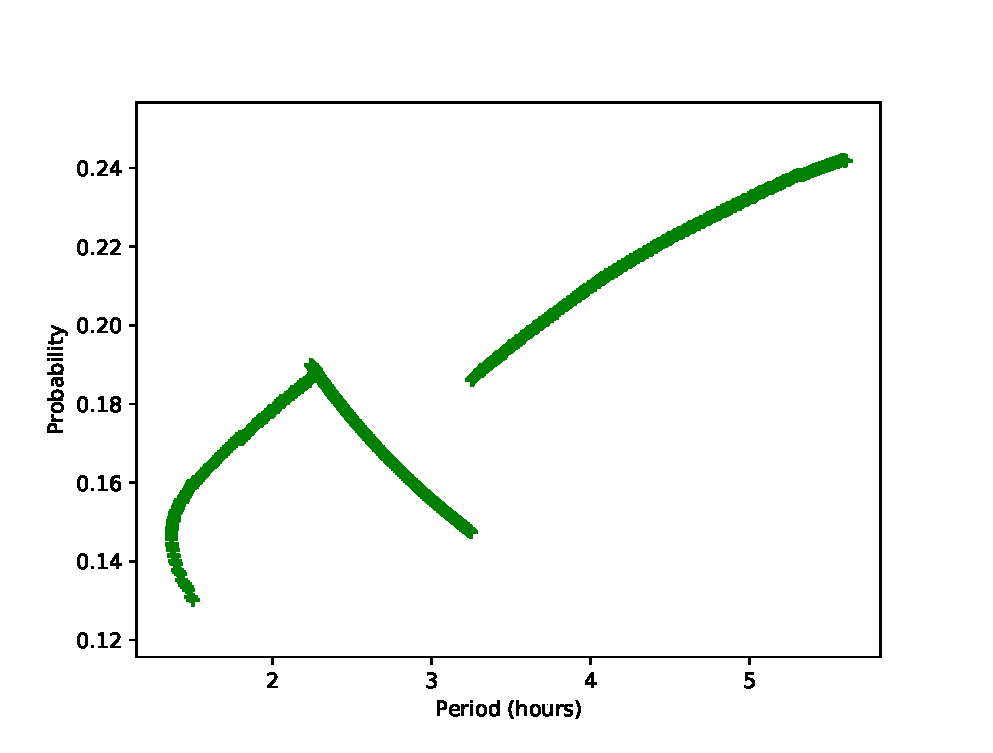
\includegraphics[scale=0.55]{./figure/p_inCV.eps}
\caption{Probability of eclipsing in CVs. The break around 3.2hours resulted by different model for CVs beyond and below the period gap.\label{fig:simpCV}}
\end{figure}

We utilized the simulation results of 5258s and 15258s as the detection rate for period under (75\% of the total number) and beyond the period gap (25\% of the total number). The fraction was taken from the DNe distribution in solar neighborhood. Besides, EP was chosen as 0.18 and 0.20 for this two types.
Similarly, the predicted number of periodic non-mCVs which "should" be detected in each counts bin is:
\begin{equation}
Np_{i}=N_i\times DR \times EP \times 667 \times \alpha	
\end{equation}
Since the sum of $Np_{i}$ was assigned as three, the $\alpha$ would be around 0.45 if we set $\rm 10^{32}~erg~s^{-1}$ (roughly corresponding 675 counts) as the upper limit of luminosity for DNe. The rationality of the limit has been proved by the DNe sample from solar neighborhood in \citep{2016ApJ...818..136X}, based on Suzaku observation. The uncertainty of this fraction comes from our limited acquaintance about XLF for DNe, and the subjective diagnostic for the phase-folded light curve. 


\section{Summary}\label{sec:summary}

1. We have discovered 23 periodic sources with 25 signal in the LW by using GL method, including 10 of them already found by LS method in \cite{2012ApJ...746..165H}. Their luminosity range locates at $\rm 10^{31}-10^{33}~erg~s^{-1} $.The general feature of these 23 sources resembles that of polars. Three of them with narrow dip are likely DNe. Two of them are determined as IP.

2.  We estimate the mass of WD from a source with great identification for Fe XXVI and Fe XXV emission lines, i.e. 0.8 $M_\odot$ for \#21(\#22) as being an IP. 

3. We provide well-constrained fraction of polars in the whole sample, i.e, 16\% as the upper limit. The estimation on fraction of non-mCVs is about 45\% while the certainty is restricted by limited appreciation about their XLF. Combined with the period distribution, we conclude that the periodic sources are mainly polars with relatively harder spectra, especially in the luminosity range that lower than $\rm 10^{32}~erg~s^{-1}$. Besides, the H sources (L>$\rm 10^{32}~erg~s^{-1}$), whose emission is mostly contributed by IPs, indicate  $M_{WD} \sim 0.8 M_\odot$, consistent with the previous result $0.8\pm 0.07 M_\odot$ in \citep{2018ApJ...853..182Y}.

4. The lower luminosity and narrow eclipsing model for orbital modulation reduced the detection rate simultaneously for periodicity. That may explain why we had no trace on non-mCVs in GCR in earlier period searching work.

5. We proved the higher detection rate, more usage of data and ignorance of observation gap for GL method compared with LS method. It is noteworthy that the shape of light curve in GL method could be modified according to different scenarios. It was applied on detection of planetary transits by using customized eclipsing model \citep{2002A&A...395..625A}. For the utility of GL method, there is still room for improvement in the future.
\\
\\

We thank Xiaojie Xu and Zhenlin Zhu for helpful discussions. This work is supported by the National Key Research and Development Program of China under grant 2017YFA0402703.

%% Appendix material should be preceded with a single \appendix command.
%% There should be a \section command for each appendix. Mark appendix
%% subsections with the same markup you use in the main body of the paper.

%% Each Appendix (indicated with \section) will be lettered A, B, C, etc.
%% The equation counter will reset when it encounters the \appendix
%% command and will number appendix equations (A1), (A2), etc. The

\bibliography{sample63}{}
\bibliographystyle{mnras}

\newpage
%\onecolumn
\appendix
\section{A brief introduction to the Gregory-Loredo algorithm}\label{GL}
The basic rules for Bayesian probabilities are the sum rule:
\begin{equation}
p(H_i|I)+p(\bar{H_i}|I)	=1
\end{equation}
And the product rule:
\begin{equation}\label{2.2}
p(H_i,D|I)=p(H_i|I)\cdot p(D|H_i,I)=p(D|I)\cdot p(H_i|D,I)
\end{equation}
From equation \ref{2.2} we could easily derive Bayes's theorem.
\begin{equation}\label{2.5} 
p(H_i|D,I)=p(H_i|I)\cdot {p(D|H_i,I)\over p(D|I)}
\end{equation}
The symbols in this work follow the same expression used in \citep{1992ApJ...398..146G}. Throughout this work, these symbols could be briefly practically understood. $H_i$ signifies model, $D$ signifies dataset, $I$ represents the ensemble of all the hypotheses considered i.e. all the model used.
GL method employs stepwise function for periodic signal. Each model has $(m+2)$ parameters: angular frequency $\omega={2\pi/P}$, P represents period; phase parameter $\phi$; and m values $r_j$, signifies the counts rate in each phase bin where j=1 to m. The following we replace $H_i$ with $M_i$ to denote the model where i represents the number of bins in stepwise model. Then the Bayes's theorem can be written as:
 \begin{equation}\label{2.11}
 p(M_i|D,I)=p(M_i|I)\cdot {p(D|M_i,I)\over p(D|I)}
 \end{equation} 
We could write $I=M_1+M_2+M_3+\cdots$, where ``+'' stands for ``or''. Thus the proposition ($M_i$,I) is true if and only if model $M_i$ is true i.e. ($M_i$,I) = $M_i$. GL method defines odds ratio to make the model comparison.
\begin{equation}\label{2.12}
O_{ij}={p(M_i|D,I)\over p(M_j|D,I)}={p(M_i|I)\over p(M_j|I)}\cdot {p(D|M_i)\over p(D|M_j)}
\end{equation}
Note that $M_1$ means constant model, $M_i$(i=2,3,4 $\cdots N_{mod}$, where $N_{mod}$ is the total number of models considered.) represents periodic model. The probabilities for each model can be deduced by \ref{2.12}
\begin{equation}\label{6}
p(M_i|D,I)=O_{i1}\cdot p(M_1|D,I)
\end{equation}
\begin{equation}\label{7}
p(M_1|D,I)={{\sum_{j=1}^{N_{mod}} p(M_j|D,I)}\over {\sum_{j=1}^{N_{mod}} O_{j1}}}
={1\over {\sum_{j=1}^{N_{mod}} O_{j1}}}	
\end{equation}
Substitute \ref{7} into \ref{6}, we got
\begin{equation}\label{2.13}
p(M_i|D,I)={O_{i1}\over {\sum_{j=1}^{N_{mod}} O_{j1}}}
\end{equation}
Then the probability that the signal is periodic is :
\begin{equation}\label{5.2}
p(M_m(m>1)|D,I)={{\sum_{m=2}^{m_{max}} O_{m1}}\over {1+\sum_{m=2}^{m_{max}} O_{m1}}}
\end{equation}
The odds ratio can be calculated by the probability for model:
\begin{equation}
O_{m1}={{p(M_m|D.I)}\over {p(M_1|D.I)}}
\end{equation}
Using Bayes's theorem shown as \ref{2.11},
\begin{equation}\label{11}
O_{m1}={{p(M_m|I)\cdot p(D|M_m)}\over {p(M_1|I)\cdot p(D|M_1)}}
\end{equation}
Following the same assignment by \citep{1992ApJ...398..146G}, we also consider the probability of periodic and aperiodic signals are the same. Then the priors for model can be written explicitly as :
\begin{equation}\label{12}
p(M_1|I)={1\over 2}	
\end{equation}
\begin{equation}\label{13}
p(M_m|I)={1\over {2\nu}}	, \quad \nu =m_{max}-1
\end{equation}
Since the essence of the algorithm is not our subject, we directly introduce the Eqn.~ 5.27 in \citep{1992ApJ...398..146G} as follows. It must be emphasized that this equation worked for the situation when the period and phase are both unknown. 
\begin{equation}\label{5.27}
\begin{split}
p(D|M_m)={{{\Delta t}^N (m-1)! N! \gamma(N+1,A_{max})T}\over{2\pi A_{max} (N+m-1)!T^{N+1} \ln(\omega_{hi}/\omega_{lo})}}\\
\times {\int_{w_{lo}}^{w_{hi}}}{{d\omega}\over{\omega}}\times {\int_0^{2\pi}d\phi{m^N\over W_m(\omega,\phi)}}	
\end{split}
\end{equation}
Substituting $m=1$ into \ref{5.27}, we got:
\begin{equation}\label{15}
p(D|M_1)={{{\Delta t}^N N!\gamma(N+1,A_{max})T}\over {A_{max}N!T^{N+1}}}
\end{equation}
Substituting \ref{12}, \ref{13}, \ref{5.27}, \ref{15} into \ref{11}, the odds ratio could be written as follows, which is the same as equation 5.28 in GL method:
\begin{equation}\label{A16}
\begin{split}
O_{m1}={1\over{2\pi \nu \ln(\omega_{hi}/\omega_{lo})}} {{N+m-1}	\choose N}^{-1}\times {\int_{w_{lo}}^{w_{hi}}}{{d\omega}\over{\omega}}\\
\times {\int_0^{2\pi}d\phi{m^N\over W_m(\omega,\phi)}} 
\end{split}
\end{equation}

In astronomical dataset, the observation always brings data gaps. For example, when the period is long and the exposure time for single observation is low, different bins may not be covered fairly. Then the initial assumptions above mentioned may fail, leading to some fake detections especially at low frequencies. In appendix B to \citep{1992ApJ...398..146G}, a solution to this problem has been proposed. They defined a weighting factor $S(\omega,\phi)$, where ${\tau_{j}(\omega,\phi)}$ signifies the exposure time in each bin:
\begin{equation}\label{A17}
S(\omega,\phi)={\prod_{j=1}^m s_j^{-n_j}}
\end{equation}
\begin{equation}
s_j(\omega,\phi)={{\tau_{j}(\omega,\phi)}\over {T/m}}
\end{equation}
Then the odds ratio should be modified as:
\begin{equation}\label{A19}
\begin{split}
O_{m1}={1\over{2\pi \nu \ln(\omega_{hi}/\omega_{lo})}} {{N+m-1}	\choose N}^{-1}\times {\int_{w_{lo}}^{w_{hi}}}{{d\omega}\over{\omega}}\\
\times {\int_0^{2\pi}d\phi{S(\omega,\phi)m^N\over W_m(\omega,\phi)}}
\end{split} 
\end{equation}
Ultimately, the probability of whether the dataset is periodic is:
\begin{equation}\label{A20}
p(periodic)={{\sum_{m=2}^{m_{max}} O_{m1}}\over {1+\sum_{m=2}^{m_{max}} O_{m1}}}
\end{equation}
The posterior probability of the frequency indicates the period of the signal:
\begin{equation}\label{A21}
O_{m1}(\omega)={1\over{2\pi \nu}} {{N+m-1}	\choose N}^{-1} \times {\int_0^{2\pi}d\phi{S(\omega,\phi)m^N\over W_m(\omega,\phi)}} 
\end{equation}
The period locates at $P=2\pi /\omega $ when $O_{m1}(\omega)$ takes the highest value.


\section{Treatment of harmonics}\label{harmonics}

\begin{figure*}
\begin{minipage}[b]{0.45\textwidth}
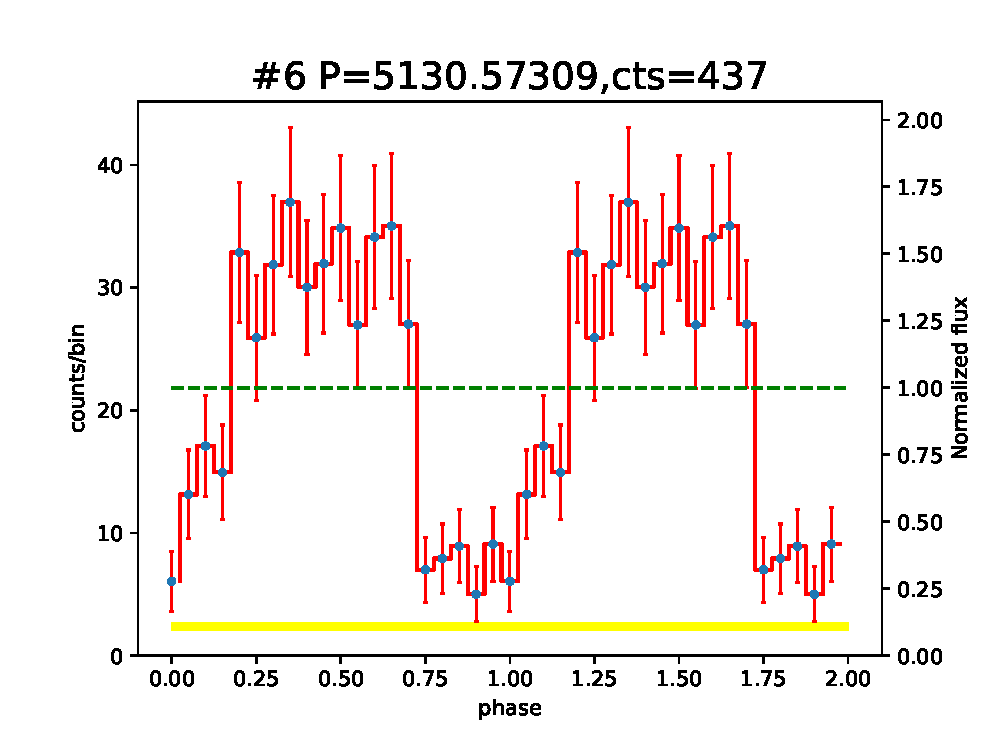
\includegraphics[width=\textwidth]{./figure/LW/pfold_lc_20.eps}
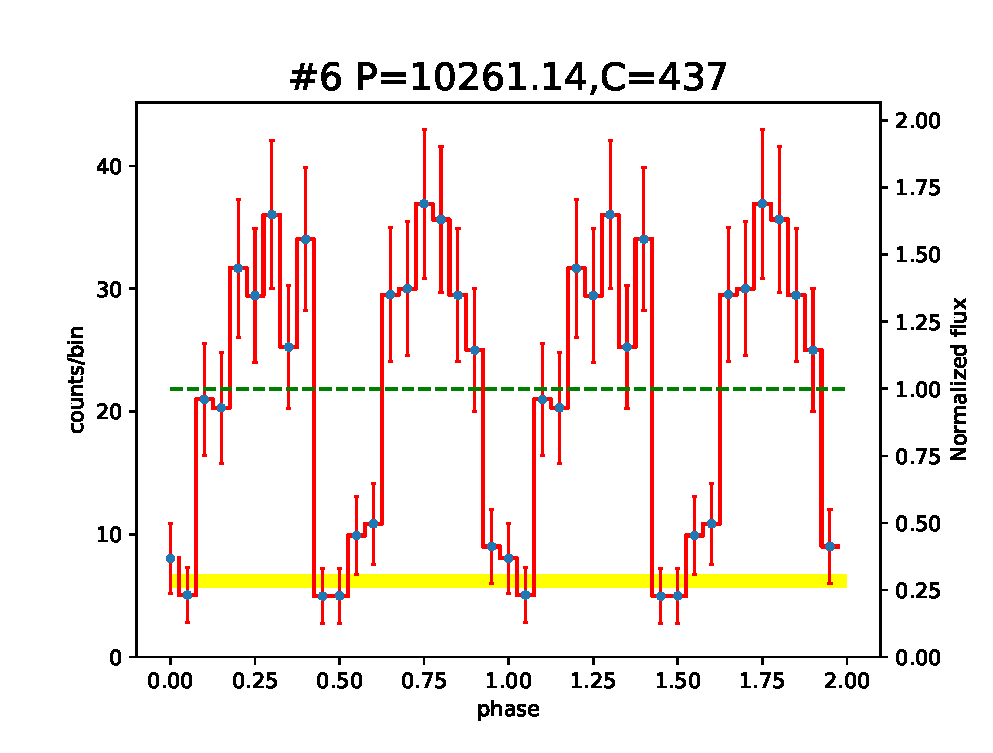
\includegraphics[width=\textwidth]{./figure/LW/pfold_lc_20_second.eps}
\end{minipage}
\begin{minipage}[b]{0.45\textwidth}
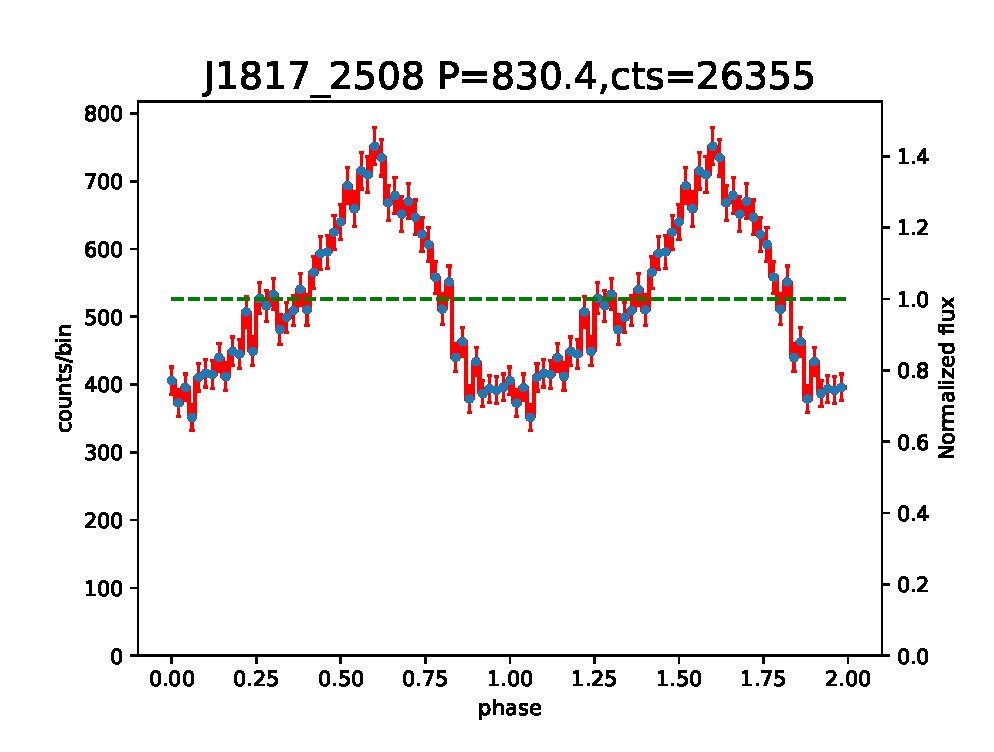
\includegraphics[width=\textwidth]{./figure/CV/pfold_lc_J1817_2508_spin_half.eps}
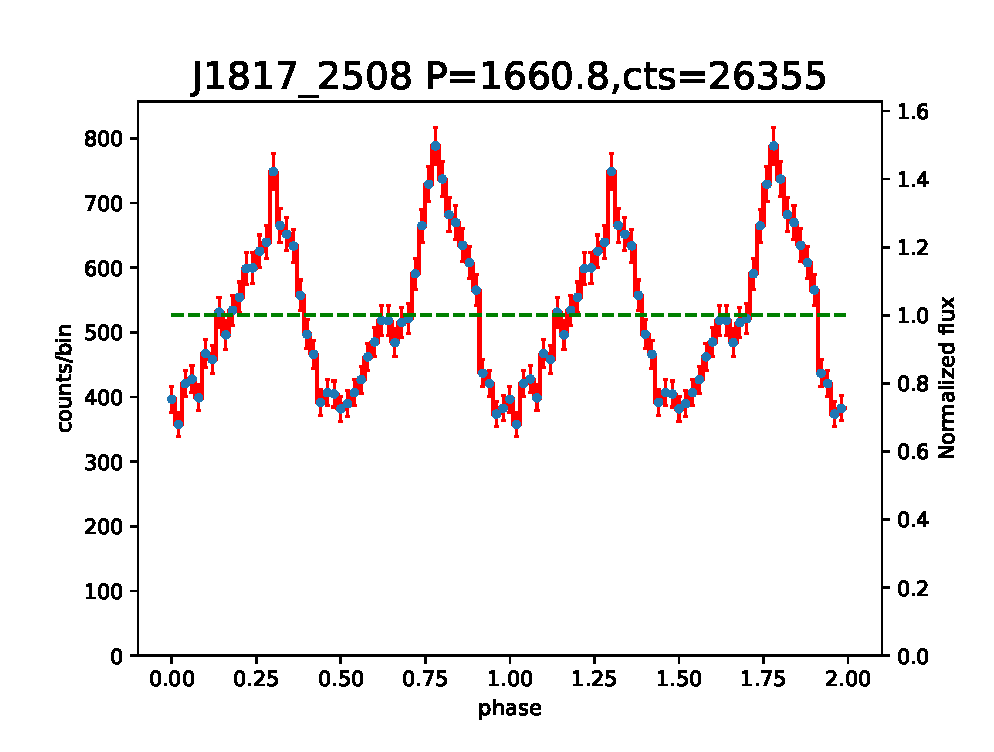
\includegraphics[width=\textwidth]{./figure/CV/pfold_lc_J1817_2508_spin.eps}
\end{minipage}
\caption{The top left and bottom left panel show the folded light curve of LW 6, at true period and second harmonics, respectively. The top right and bottom right panel display the folded light curve of J1817-2508. While for this source, the double-peaked shape (bottom right) at 1660s are the real signal of rotation. \label{fig:6thfig}}
\end{figure*}
\indent
To determine the intrinsic period, whether it's rotation period or orbital period, from primary period and harmonics, we should not focus on data and the significance of signals. In that the intensities of signals could not reflect the authenticity of the signal precisely. For the sake of  identification, the physical mechanism of period in CVs must be introduced. 

Here we take the 6th signal as an illustration, the phase-folded light curve of primary period and second harmonic show classic  single-peak shape and double-peak shape, see the left two panels in Figure \ref{fig:6thfig}. For comparison, we also present the phase-folded light curve of J1817-2508 based on XMM-Newton observations (obsID=0601270301).
We processed the EPIC PN and MOS data with the standard tool \emph{emchain} and \emph{epchain} in SAS v18.0.0. Similarly, the arrival time of photons were corrected at the Solar barycenter  by applying the task \emph{barycen}.
Then we extract the 0.2-10 keV light curve and folded it from PN data for it has the largest effective area.

 The J1817-2508, which was also called IGR J18173-2509, has been determined with pulsation at 830.70s from Swift-XRT detection. Then the signal of 1660s has also been detected from Chandra observation \citep{2009ATel.2354....1N} and the optical period of 1690s \citep{2012A&A...542A..22B}. All the above strongly suggests that the true spin period is about 1660s, twice the first detected X-ray period, even though the two peaks in modulation are quite similar, as shown in the lower right panel in Figure \ref{fig:6thfig}.
 
 The properties of J1817-2508 indicates that phase-folded light curve could be extremely deceptive under the circumstances that sources with symmetric dipole structure. We could not precisely determine the true rotation period without optical observations. However, the physical origins of periodic signals may provide additional constrains on the judgement. The double-peak shape only happens in IP with accretion column model. The two poles where accretion region lied on, would be the brightest. When we look at them at a specific angle, the two poles alternatively flitting across the face of WDs, and then produce the double-peaked pulsation. In this kind of situation, the modulation period must be the rotation period of WDs, mostly under one hour. While the second harmonics of our sources, are mostly beyond 3 hours. It would be a risky assumption if these harmonics served as spin period. On the other hand, despite the WDs in polars may have such long rotation period from synchronization effect, their accretion stream always falls on the single pole, emitting most of the soft X-ray radiation. Then the double-peaked pulsation are almost impossible. 
 
 In conclusion, according to the length of period in our sources, we took the single-peaked signal, normally the shortest period, as the real orbital period. The double-peaked shape in harmonics are treated as spurious signal. 
%\clearpage
%\newpage
\section{Figures for periodic X-ray sources}\label{appen:fig}
  \begin{figure*}
    \centering
    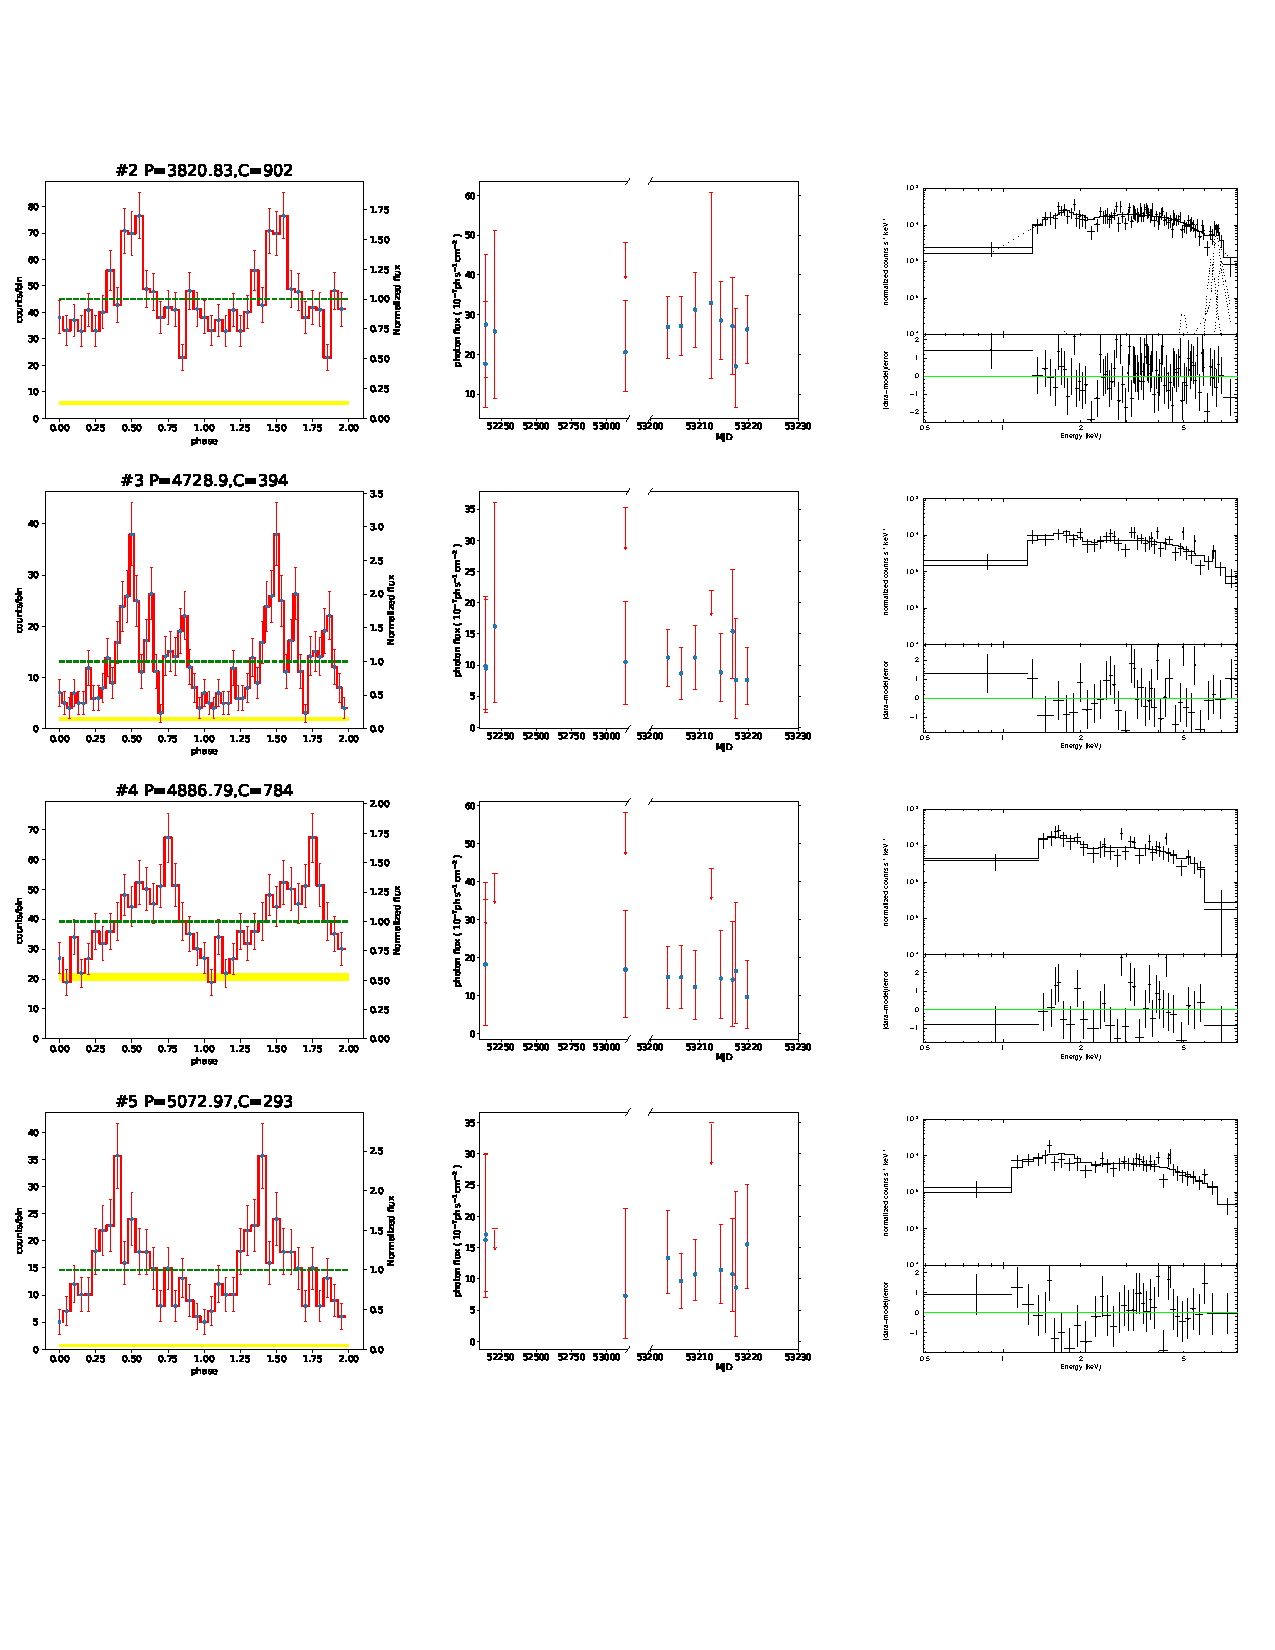
\includegraphics[page=1,scale=0.90,trim=0 100 0 20,clip]{plot_figure_LW.pdf}
    \caption{The phase-folded light curve (left) , the long-term, inter-observation light curve (middle) and the spectra (right) for all the source in Table \ref{tab:src}, similar to Figure \ref{fig:pCV_sample_1}. 
    \label{fig:Figure_p}}
  \end{figure*}
  
  \begin{figure*}
%    \ContinuedFloat
%    \captionsetup{list=off,format=cont}
    \centering
    \includegraphics[page=2,scale=0.90,trim=0 100 0 20,clip]{plot_figure_LW.pdf}
    \caption{First figure continued}
  \end{figure*}

  \begin{figure*}
%  \ContinuedFloat
%  \captionsetup{list=off,format=cont}
    \centering
    \includegraphics[page=3,scale=0.90,trim=0 100 0 20,clip]{plot_figure_LW.pdf}
    \caption{First figure continued}
  \end{figure*}
  
   \begin{figure*}
%  \ContinuedFloat
%  \captionsetup{list=off,format=cont}
    \centering
    \includegraphics[page=4,scale=0.90,trim=0 100 0 20,clip]{plot_figure_LW.pdf}
    \caption{First figure continued}
  \end{figure*}
  
  \begin{figure*}
%  \ContinuedFloat
%  \captionsetup{list=off,format=cont}
    \centering
    \includegraphics[page=5,scale=0.90,trim=0 100 0 20,clip]{plot_figure_LW.pdf}
    \caption{First figure continued}
  \end{figure*}
  
  \begin{figure*}
%  \ContinuedFloat
%  \captionsetup{list=off,format=cont}
    \centering
    \includegraphics[page=6,scale=0.90,trim=0 100 0 20,clip]{plot_figure_LW.pdf}
    \caption{First figure continued}
  \end{figure*}
  
   \begin{figure*}
%  \ContinuedFloat
%  \captionsetup{list=off,format=cont}
    \centering
    \includegraphics[page=7,scale=0.90,trim=0 550 0 20,clip]{plot_figure_LW.pdf}
    \caption{First figure continued}
  \end{figure*}

%% For this sample we use BibTeX plus aasjournals.bst to generate the
%% the bibliography. The sample63.bib file was populated from ADS. To
%% get the citations to show in the compiled file do the following:
%%
%% pdflatex sample63.tex
%% bibtext sample63
%% pdflatex sample63.tex
%% pdflatex sample63.tex


\end{document}

% End of file `sample63.tex'.
